\documentclass[conference]{IEEEtran}
% Every number in this paper is a macro defined in generated/numbers.tex, which is produced by
% paper/make_assets.py from results/raw/ only. Tables are \input from generated/tab_*.tex.
\usepackage{amsmath,amssymb,amsthm}
\usepackage{graphicx}
\usepackage{booktabs}
\usepackage{url}
\usepackage[hidelinks]{hyperref}
% AUTO-GENERATED by paper/make_assets.py from results/raw/ -- do not edit
\newcommand{\EeightMaxShareGap}{0.09}  % results/raw/e8_privacy/runs.csv
\newcommand{\EeightSig}{0}  % results/raw/stats/e8_privacy.csv
\newcommand{\EeightSigWeightsWorse}{0}  % results/raw/stats/e8_privacy.csv
\newcommand{\EeightTests}{6}  % results/raw/stats/e8_privacy.csv
\newcommand{\EeightVotesBeatRandom}{6}  % results/raw/stats/e8_privacy.csv
\newcommand{\EeightVotesRandomTests}{6}  % results/raw/stats/e8_privacy.csv
\newcommand{\EelevenBLegacyBeta}{8}  % results/raw/e11_adaptive/best.json
\newcommand{\EelevenBSgFull}{8}  % results/raw/e11_adaptive/best.json
\newcommand{\EelevenBSgNoCap}{8}  % results/raw/e11_adaptive/best.json
\newcommand{\EelevenBSgNoCusum}{8}  % results/raw/e11_adaptive/best.json
\newcommand{\EelevenBSgNoTwoTimescale}{8}  % results/raw/e11_adaptive/best.json
\newcommand{\EelevenBSgNone}{8}  % results/raw/e11_adaptive/best.json
\newcommand{\EelevenFOneLegacyBeta}{0.00}  % results/raw/e11_adaptive/runs.csv
\newcommand{\EelevenFOneSgFull}{0.24}  % results/raw/e11_adaptive/runs.csv
\newcommand{\EelevenFOneSgNoCap}{0.24}  % results/raw/e11_adaptive/runs.csv
\newcommand{\EelevenFOneSgNoCusum}{0.00}  % results/raw/e11_adaptive/runs.csv
\newcommand{\EelevenFOneSgNoTwoTimescale}{0.13}  % results/raw/e11_adaptive/runs.csv
\newcommand{\EelevenFOneSgNone}{0.00}  % results/raw/e11_adaptive/runs.csv
\newcommand{\EelevenInvalidLegacyBeta}{0.0023}  % results/raw/e11_adaptive/runs.csv
\newcommand{\EelevenInvalidSgFull}{0.0007}  % results/raw/e11_adaptive/runs.csv
\newcommand{\EelevenInvalidSgNoCap}{0.0007}  % results/raw/e11_adaptive/runs.csv
\newcommand{\EelevenInvalidSgNoCusum}{0.0011}  % results/raw/e11_adaptive/runs.csv
\newcommand{\EelevenInvalidSgNoTwoTimescale}{0.0008}  % results/raw/e11_adaptive/runs.csv
\newcommand{\EelevenInvalidSgNone}{0.0015}  % results/raw/e11_adaptive/runs.csv
\newcommand{\EelevenRateLegacyBeta}{0.50}  % results/raw/e11_adaptive/best.json
\newcommand{\EelevenRateSgFull}{0.50}  % results/raw/e11_adaptive/best.json
\newcommand{\EelevenRateSgNoCap}{0.50}  % results/raw/e11_adaptive/best.json
\newcommand{\EelevenRateSgNoCusum}{0.50}  % results/raw/e11_adaptive/best.json
\newcommand{\EelevenRateSgNoTwoTimescale}{0.30}  % results/raw/e11_adaptive/best.json
\newcommand{\EelevenRateSgNone}{0.30}  % results/raw/e11_adaptive/best.json
\newcommand{\EelevenRejectLegacyBeta}{0.000}  % results/raw/e11_adaptive/runs.csv
\newcommand{\EelevenRejectSgFull}{0.001}  % results/raw/e11_adaptive/runs.csv
\newcommand{\EelevenRejectSgNoCap}{0.000}  % results/raw/e11_adaptive/runs.csv
\newcommand{\EelevenRejectSgNoCusum}{0.000}  % results/raw/e11_adaptive/runs.csv
\newcommand{\EelevenRejectSgNoTwoTimescale}{0.000}  % results/raw/e11_adaptive/runs.csv
\newcommand{\EelevenRejectSgNone}{0.000}  % results/raw/e11_adaptive/runs.csv
\newcommand{\EelevenSgBelowBoundBreach}{0}  % results/raw/e11_adaptive/runs.csv
\newcommand{\EelevenSgBelowBoundBreachCp}{2.5}  % results/raw/e11_adaptive/runs.csv
\newcommand{\EelevenSgBelowBoundRuns}{120}  % results/raw/e11_adaptive/runs.csv
\newcommand{\EfifteenBatchesCentiDirOne}{never}  % results/raw/e15_weight_recovery/summary.csv
\newcommand{\EfifteenBatchesCentiDirThree}{never}  % results/raw/e15_weight_recovery/summary.csv
\newcommand{\EfifteenBatchesCentiDirTwo}{never}  % results/raw/e15_weight_recovery/summary.csv
\newcommand{\EfifteenBatchesCentiDirZero}{4}  % results/raw/e15_weight_recovery/summary.csv
\newcommand{\EfifteenBatchesCentiInvOne}{4}  % results/raw/e15_weight_recovery/summary.csv
\newcommand{\EfifteenBatchesCentiInvThree}{4}  % results/raw/e15_weight_recovery/summary.csv
\newcommand{\EfifteenBatchesCentiInvTwo}{4}  % results/raw/e15_weight_recovery/summary.csv
\newcommand{\EfifteenBatchesCentiInvZero}{4}  % results/raw/e15_weight_recovery/summary.csv
\newcommand{\EfifteenBatchesMilliDirOne}{never}  % results/raw/e15_weight_recovery/summary.csv
\newcommand{\EfifteenBatchesMilliDirThree}{never}  % results/raw/e15_weight_recovery/summary.csv
\newcommand{\EfifteenBatchesMilliDirTwo}{never}  % results/raw/e15_weight_recovery/summary.csv
\newcommand{\EfifteenBatchesMilliDirZero}{4}  % results/raw/e15_weight_recovery/summary.csv
\newcommand{\EfifteenBatchesMilliInvOne}{4}  % results/raw/e15_weight_recovery/summary.csv
\newcommand{\EfifteenBatchesMilliInvThree}{4}  % results/raw/e15_weight_recovery/summary.csv
\newcommand{\EfifteenBatchesMilliInvTwo}{4}  % results/raw/e15_weight_recovery/summary.csv
\newcommand{\EfifteenBatchesMilliInvZero}{4}  % results/raw/e15_weight_recovery/summary.csv
\newcommand{\EfifteenErrDirOne}{5e-01}  % results/raw/e15_weight_recovery/summary.csv
\newcommand{\EfifteenErrDirThree}{2e+00}  % results/raw/e15_weight_recovery/summary.csv
\newcommand{\EfifteenErrDirTwo}{1e+00}  % results/raw/e15_weight_recovery/summary.csv
\newcommand{\EfifteenErrDirZero}{1e-07}  % results/raw/e15_weight_recovery/summary.csv
\newcommand{\EfifteenErrInvOne}{5e-06}  % results/raw/e15_weight_recovery/summary.csv
\newcommand{\EfifteenErrInvThree}{2e-05}  % results/raw/e15_weight_recovery/summary.csv
\newcommand{\EfifteenErrInvTwo}{1e-05}  % results/raw/e15_weight_recovery/summary.csv
\newcommand{\EfifteenErrInvZero}{1e-07}  % results/raw/e15_weight_recovery/summary.csv
\newcommand{\EfifteenInvBatchesMax}{7}  % results/raw/e15_weight_recovery/summary.csv
\newcommand{\EfifteenInvErrMax}{2e-05}  % results/raw/e15_weight_recovery/summary.csv
\newcommand{\EfifteenRecoveredCentiDirOne}{0}  % results/raw/e15_weight_recovery/summary.csv
\newcommand{\EfifteenRecoveredCentiDirThree}{0}  % results/raw/e15_weight_recovery/summary.csv
\newcommand{\EfifteenRecoveredCentiDirTwo}{0}  % results/raw/e15_weight_recovery/summary.csv
\newcommand{\EfifteenRecoveredCentiDirZero}{30}  % results/raw/e15_weight_recovery/summary.csv
\newcommand{\EfifteenRecoveredCentiInvOne}{30}  % results/raw/e15_weight_recovery/summary.csv
\newcommand{\EfifteenRecoveredCentiInvThree}{30}  % results/raw/e15_weight_recovery/summary.csv
\newcommand{\EfifteenRecoveredCentiInvTwo}{30}  % results/raw/e15_weight_recovery/summary.csv
\newcommand{\EfifteenRecoveredCentiInvZero}{30}  % results/raw/e15_weight_recovery/summary.csv
\newcommand{\EfifteenRecoveredMilliDirOne}{0}  % results/raw/e15_weight_recovery/summary.csv
\newcommand{\EfifteenRecoveredMilliDirThree}{0}  % results/raw/e15_weight_recovery/summary.csv
\newcommand{\EfifteenRecoveredMilliDirTwo}{0}  % results/raw/e15_weight_recovery/summary.csv
\newcommand{\EfifteenRecoveredMilliDirZero}{30}  % results/raw/e15_weight_recovery/summary.csv
\newcommand{\EfifteenRecoveredMilliInvOne}{30}  % results/raw/e15_weight_recovery/summary.csv
\newcommand{\EfifteenRecoveredMilliInvThree}{30}  % results/raw/e15_weight_recovery/summary.csv
\newcommand{\EfifteenRecoveredMilliInvTwo}{30}  % results/raw/e15_weight_recovery/summary.csv
\newcommand{\EfifteenRecoveredMilliInvZero}{30}  % results/raw/e15_weight_recovery/summary.csv
\newcommand{\EfifteenSatMaxPct}{8.48}  % results/raw/e15_weight_recovery/summary.csv
\newcommand{\EfifteenTrials}{30}  % results/raw/e15_weight_recovery/summary.csv
\newcommand{\EfiveBigCensoredPct}{77}  % results/raw/e5_scale/runs.csv
\newcommand{\EfiveBigFOne}{0.42}  % results/raw/e5_scale/runs.csv
\newcommand{\EfiveBigMem}{35}  % results/raw/e5_scale/runs.csv
\newcommand{\EfiveBigWall}{8.4}  % results/raw/e5_scale/runs.csv
\newcommand{\EfiveMaxNodes}{1024}  % results/raw/e5_scale/runs.csv
\newcommand{\EfiveMinFOne}{0.06}  % results/raw/e5_scale/runs.csv
\newcommand{\EfiveSeeds}{30}  % results/raw/e5_scale/runs.csv
\newcommand{\EfiveSmallCensoredPct}{0}  % results/raw/e5_scale/runs.csv
\newcommand{\EfourBandMaxFlip}{1e-08}  % results/raw/e4_he/band.csv
\newcommand{\EfourBandMinSafe}{1e-08}  % results/raw/e4_he/band.csv
\newcommand{\EfourBandOne}{0.0e+00}  % results/raw/e4_he/decisions.csv
\newcommand{\EfourBandThree}{0.0e+00}  % results/raw/e4_he/decisions.csv
\newcommand{\EfourBandTwo}{0.0e+00}  % results/raw/e4_he/decisions.csv
\newcommand{\EfourBandZero}{0.0e+00}  % results/raw/e4_he/decisions.csv
\newcommand{\EfourConsDecisionsThree}{4800}  % results/raw/e4_he/consensus.csv
\newcommand{\EfourConsDecisionsZero}{8000}  % results/raw/e4_he/consensus.csv
\newcommand{\EfourConsFlipsThree}{0}  % results/raw/e4_he/consensus.csv
\newcommand{\EfourConsFlipsThreeCp}{0.062}  % results/raw/e4_he/consensus.csv
\newcommand{\EfourConsFlipsZero}{0}  % results/raw/e4_he/consensus.csv
\newcommand{\EfourConsFlipsZeroCp}{0.037}  % results/raw/e4_he/consensus.csv
\newcommand{\EfourConsWallPlain}{0.26}  % results/raw/e4_he/consensus.csv
\newcommand{\EfourConsWallThree}{422}  % results/raw/e4_he/consensus.csv
\newcommand{\EfourConsWallZero}{32}  % results/raw/e4_he/consensus.csv
\newcommand{\EfourDecisionsOne}{3360}  % results/raw/e4_he/decisions.csv
\newcommand{\EfourDecisionsThree}{3360}  % results/raw/e4_he/decisions.csv
\newcommand{\EfourDecisionsTotal}{13440}  % results/raw/e4_he/decisions.csv
\newcommand{\EfourDecisionsTwo}{3360}  % results/raw/e4_he/decisions.csv
\newcommand{\EfourDecisionsZero}{3360}  % results/raw/e4_he/decisions.csv
\newcommand{\EfourFlipsOutOne}{0}  % results/raw/e4_he/decisions.csv
\newcommand{\EfourFlipsOutThree}{0}  % results/raw/e4_he/decisions.csv
\newcommand{\EfourFlipsOutTwo}{0}  % results/raw/e4_he/decisions.csv
\newcommand{\EfourFlipsOutZero}{0}  % results/raw/e4_he/decisions.csv
\newcommand{\EfourFlipsTotal}{0}  % results/raw/e4_he/decisions.csv
\newcommand{\EfourFlipsTotalCp}{0.022}  % results/raw/e4_he/decisions.csv
\newcommand{\EfourLeakErrMax}{8e-06}  % results/raw/e4_he/leakage.csv
\newcommand{\EfourMsOne}{221}  % results/raw/e4_he/timings.csv
\newcommand{\EfourMsThree}{451}  % results/raw/e4_he/timings.csv
\newcommand{\EfourMsTwo}{304}  % results/raw/e4_he/timings.csv
\newcommand{\EfourMsZero}{38}  % results/raw/e4_he/timings.csv
\newcommand{\EfourSatMaxPct}{0.15}  % results/raw/e4_he/leakage.csv
\newcommand{\EfourteenBudgetViolations}{0}  % results/raw/e14_baselines/calibration.csv
\newcommand{\EfourteenCells}{6}  % results/raw/e14_baselines/runs.csv
\newcommand{\EfourteenCuAdB}{8}  % results/raw/e14_baselines/best.json
\newcommand{\EfourteenCuAdFOne}{0.37}  % results/raw/e14_baselines/runs.csv
\newcommand{\EfourteenCuAdIc}{0.0000}  % results/raw/e14_baselines/runs.csv
\newcommand{\EfourteenCuBfiFOne}{0.94}  % results/raw/e14_baselines/runs.csv
\newcommand{\EfourteenCuBudgetMetFive}{yes}  % results/raw/e14_baselines/calibration.csv
\newcommand{\EfourteenCuBudgetMetTen}{yes}  % results/raw/e14_baselines/calibration.csv
\newcommand{\EfourteenCuBudgetMetTwo}{yes}  % results/raw/e14_baselines/calibration.csv
\newcommand{\EfourteenCuCraFOne}{0.99}  % results/raw/e14_baselines/runs.csv
\newcommand{\EfourteenCuDelay}{5.5}  % results/raw/e14_baselines/runs.csv
\newcommand{\EfourteenCuDelayBetterSg}{0}  % results/raw/stats/e14_baselines.csv
\newcommand{\EfourteenCuDelayWorseSg}{0}  % results/raw/stats/e14_baselines.csv
\newcommand{\EfourteenCuFOneBetterSg}{3}  % results/raw/stats/e14_baselines.csv
\newcommand{\EfourteenCuFOneTenF}{0.63}  % results/raw/e14_baselines/runs.csv
\newcommand{\EfourteenCuFOneTenM}{0.73}  % results/raw/e14_baselines/runs.csv
\newcommand{\EfourteenCuFOneTwoF}{0.80}  % results/raw/e14_baselines/runs.csv
\newcommand{\EfourteenCuFOneTwoM}{0.86}  % results/raw/e14_baselines/runs.csv
\newcommand{\EfourteenCuFOneWorseSg}{2}  % results/raw/stats/e14_baselines.csv
\newcommand{\EfourteenCuFlagged}{7.4}  % results/raw/e14_baselines/runs.csv
\newcommand{\EfourteenCuFlaggedTenF}{192.4}  % results/raw/e14_baselines/runs.csv
\newcommand{\EfourteenCuFlaggedTenM}{11.6}  % results/raw/e14_baselines/runs.csv
\newcommand{\EfourteenCuFlaggedTwoF}{0.0}  % results/raw/e14_baselines/runs.csv
\newcommand{\EfourteenCuFlaggedTwoM}{8.2}  % results/raw/e14_baselines/runs.csv
\newcommand{\EfourteenCuFq}{0.47}  % results/raw/e14_baselines/runs.csv
\newcommand{\EfourteenCuFqTenF}{11.82}  % results/raw/e14_baselines/runs.csv
\newcommand{\EfourteenCuFqTenM}{0.73}  % results/raw/e14_baselines/runs.csv
\newcommand{\EfourteenCuFqTests}{7}  % results/raw/stats/e14_baselines.csv
\newcommand{\EfourteenCuFqTwoF}{0.00}  % results/raw/e14_baselines/runs.csv
\newcommand{\EfourteenCuFqTwoM}{0.52}  % results/raw/e14_baselines/runs.csv
\newcommand{\EfourteenCuFqWorseSg}{3}  % results/raw/stats/e14_baselines.csv
\newcommand{\EfourteenCuIc}{0.0000}  % results/raw/e14_baselines/runs.csv
\newcommand{\EfourteenCuLieDelay}{0.7}  % results/raw/e14_baselines/runs.csv
\newcommand{\EfourteenCuLieFOne}{0.98}  % results/raw/e14_baselines/runs.csv
\newcommand{\EfourteenCuNmaFOne}{0.95}  % results/raw/e14_baselines/runs.csv
\newcommand{\EfourteenCuStealthFOne}{0.80}  % results/raw/e14_baselines/runs.csv
\newcommand{\EfourteenCuStealthPrec}{0.96}  % results/raw/e14_baselines/runs.csv
\newcommand{\EfourteenCuStealthRec}{0.68}  % results/raw/e14_baselines/runs.csv
\newcommand{\EfourteenCuVr}{0.002}  % results/raw/e14_baselines/runs.csv
\newcommand{\EfourteenCuVrBetterSg}{3}  % results/raw/stats/e14_baselines.csv
\newcommand{\EfourteenEwAdB}{8}  % results/raw/e14_baselines/best.json
\newcommand{\EfourteenEwAdFOne}{0.25}  % results/raw/e14_baselines/runs.csv
\newcommand{\EfourteenEwAdIc}{0.0000}  % results/raw/e14_baselines/runs.csv
\newcommand{\EfourteenEwBfiFOne}{0.94}  % results/raw/e14_baselines/runs.csv
\newcommand{\EfourteenEwBudgetMetFive}{yes}  % results/raw/e14_baselines/calibration.csv
\newcommand{\EfourteenEwBudgetMetTen}{yes}  % results/raw/e14_baselines/calibration.csv
\newcommand{\EfourteenEwBudgetMetTwo}{yes}  % results/raw/e14_baselines/calibration.csv
\newcommand{\EfourteenEwCraFOne}{0.99}  % results/raw/e14_baselines/runs.csv
\newcommand{\EfourteenEwDelay}{5.0}  % results/raw/e14_baselines/runs.csv
\newcommand{\EfourteenEwDelayBetterSg}{2}  % results/raw/stats/e14_baselines.csv
\newcommand{\EfourteenEwDelayWorseSg}{0}  % results/raw/stats/e14_baselines.csv
\newcommand{\EfourteenEwFOneBetterSg}{3}  % results/raw/stats/e14_baselines.csv
\newcommand{\EfourteenEwFOneTenF}{0.64}  % results/raw/e14_baselines/runs.csv
\newcommand{\EfourteenEwFOneTenM}{0.72}  % results/raw/e14_baselines/runs.csv
\newcommand{\EfourteenEwFOneTwoF}{0.80}  % results/raw/e14_baselines/runs.csv
\newcommand{\EfourteenEwFOneTwoM}{0.86}  % results/raw/e14_baselines/runs.csv
\newcommand{\EfourteenEwFOneWorseSg}{3}  % results/raw/stats/e14_baselines.csv
\newcommand{\EfourteenEwFlagged}{12.0}  % results/raw/e14_baselines/runs.csv
\newcommand{\EfourteenEwFlaggedTenF}{178.6}  % results/raw/e14_baselines/runs.csv
\newcommand{\EfourteenEwFlaggedTenM}{12.2}  % results/raw/e14_baselines/runs.csv
\newcommand{\EfourteenEwFlaggedTwoF}{0.0}  % results/raw/e14_baselines/runs.csv
\newcommand{\EfourteenEwFlaggedTwoM}{9.0}  % results/raw/e14_baselines/runs.csv
\newcommand{\EfourteenEwFq}{0.73}  % results/raw/e14_baselines/runs.csv
\newcommand{\EfourteenEwFqTenF}{11.41}  % results/raw/e14_baselines/runs.csv
\newcommand{\EfourteenEwFqTenM}{0.83}  % results/raw/e14_baselines/runs.csv
\newcommand{\EfourteenEwFqTests}{7}  % results/raw/stats/e14_baselines.csv
\newcommand{\EfourteenEwFqTwoF}{0.00}  % results/raw/e14_baselines/runs.csv
\newcommand{\EfourteenEwFqTwoM}{0.52}  % results/raw/e14_baselines/runs.csv
\newcommand{\EfourteenEwFqWorseSg}{7}  % results/raw/stats/e14_baselines.csv
\newcommand{\EfourteenEwIc}{0.0000}  % results/raw/e14_baselines/runs.csv
\newcommand{\EfourteenEwLieDelay}{0.3}  % results/raw/e14_baselines/runs.csv
\newcommand{\EfourteenEwLieFOne}{0.97}  % results/raw/e14_baselines/runs.csv
\newcommand{\EfourteenEwNmaFOne}{0.95}  % results/raw/e14_baselines/runs.csv
\newcommand{\EfourteenEwStealthFOne}{0.79}  % results/raw/e14_baselines/runs.csv
\newcommand{\EfourteenEwStealthPrec}{0.94}  % results/raw/e14_baselines/runs.csv
\newcommand{\EfourteenEwStealthRec}{0.69}  % results/raw/e14_baselines/runs.csv
\newcommand{\EfourteenEwVr}{0.002}  % results/raw/e14_baselines/runs.csv
\newcommand{\EfourteenEwVrBetterSg}{4}  % results/raw/stats/e14_baselines.csv
\newcommand{\EfourteenGridBudget}{25}  % results/raw/e14_baselines/calibration.csv
\newcommand{\EfourteenLbAdB}{8}  % results/raw/e14_baselines/best.json
\newcommand{\EfourteenLbAdFOne}{0.00}  % results/raw/e14_baselines/runs.csv
\newcommand{\EfourteenLbAdIc}{0.0023}  % results/raw/e14_baselines/runs.csv
\newcommand{\EfourteenLbBfiFOne}{0.00}  % results/raw/e14_baselines/runs.csv
\newcommand{\EfourteenLbCraFOne}{1.00}  % results/raw/e14_baselines/runs.csv
\newcommand{\EfourteenLbDelay}{300.0}  % results/raw/e14_baselines/runs.csv
\newcommand{\EfourteenLbDelayBetterSg}{0}  % results/raw/stats/e14_baselines.csv
\newcommand{\EfourteenLbDelayWorseSg}{6}  % results/raw/stats/e14_baselines.csv
\newcommand{\EfourteenLbFOneBetterSg}{0}  % results/raw/stats/e14_baselines.csv
\newcommand{\EfourteenLbFOneTenF}{0.00}  % results/raw/e14_baselines/runs.csv
\newcommand{\EfourteenLbFOneTenM}{0.00}  % results/raw/e14_baselines/runs.csv
\newcommand{\EfourteenLbFOneTwoF}{0.00}  % results/raw/e14_baselines/runs.csv
\newcommand{\EfourteenLbFOneTwoM}{0.00}  % results/raw/e14_baselines/runs.csv
\newcommand{\EfourteenLbFOneWorseSg}{6}  % results/raw/stats/e14_baselines.csv
\newcommand{\EfourteenLbFlagged}{0.0}  % results/raw/e14_baselines/runs.csv
\newcommand{\EfourteenLbFlaggedTenF}{0.0}  % results/raw/e14_baselines/runs.csv
\newcommand{\EfourteenLbFlaggedTenM}{0.0}  % results/raw/e14_baselines/runs.csv
\newcommand{\EfourteenLbFlaggedTwoF}{0.0}  % results/raw/e14_baselines/runs.csv
\newcommand{\EfourteenLbFlaggedTwoM}{0.0}  % results/raw/e14_baselines/runs.csv
\newcommand{\EfourteenLbFq}{0.00}  % results/raw/e14_baselines/runs.csv
\newcommand{\EfourteenLbFqTenF}{0.00}  % results/raw/e14_baselines/runs.csv
\newcommand{\EfourteenLbFqTenM}{0.00}  % results/raw/e14_baselines/runs.csv
\newcommand{\EfourteenLbFqTests}{7}  % results/raw/stats/e14_baselines.csv
\newcommand{\EfourteenLbFqTwoF}{0.00}  % results/raw/e14_baselines/runs.csv
\newcommand{\EfourteenLbFqTwoM}{0.00}  % results/raw/e14_baselines/runs.csv
\newcommand{\EfourteenLbFqWorseSg}{0}  % results/raw/stats/e14_baselines.csv
\newcommand{\EfourteenLbIc}{0.0000}  % results/raw/e14_baselines/runs.csv
\newcommand{\EfourteenLbLieDelay}{300.0}  % results/raw/e14_baselines/runs.csv
\newcommand{\EfourteenLbLieFOne}{0.00}  % results/raw/e14_baselines/runs.csv
\newcommand{\EfourteenLbNmaFOne}{0.00}  % results/raw/e14_baselines/runs.csv
\newcommand{\EfourteenLbStealthFOne}{0.00}  % results/raw/e14_baselines/runs.csv
\newcommand{\EfourteenLbStealthPrec}{0.00}  % results/raw/e14_baselines/runs.csv
\newcommand{\EfourteenLbStealthRec}{0.00}  % results/raw/e14_baselines/runs.csv
\newcommand{\EfourteenLbVr}{0.044}  % results/raw/e14_baselines/runs.csv
\newcommand{\EfourteenLbVrBetterSg}{0}  % results/raw/stats/e14_baselines.csv
\newcommand{\EfourteenLieLossMax}{0.028}  % results/raw/stats/e14_baselines.csv
\newcommand{\EfourteenLieTests}{9}  % results/raw/stats/e14_baselines.csv
\newcommand{\EfourteenLieWorse}{7}  % results/raw/stats/e14_baselines.csv
\newcommand{\EfourteenLtAdB}{8}  % results/raw/e14_baselines/best.json
\newcommand{\EfourteenLtAdFOne}{0.00}  % results/raw/e14_baselines/runs.csv
\newcommand{\EfourteenLtAdIc}{0.0023}  % results/raw/e14_baselines/runs.csv
\newcommand{\EfourteenLtBfiFOne}{1.00}  % results/raw/e14_baselines/runs.csv
\newcommand{\EfourteenLtBudgetMetFive}{yes}  % results/raw/e14_baselines/calibration.csv
\newcommand{\EfourteenLtBudgetMetTen}{yes}  % results/raw/e14_baselines/calibration.csv
\newcommand{\EfourteenLtBudgetMetTwo}{yes}  % results/raw/e14_baselines/calibration.csv
\newcommand{\EfourteenLtCraFOne}{1.00}  % results/raw/e14_baselines/runs.csv
\newcommand{\EfourteenLtDelay}{300.0}  % results/raw/e14_baselines/runs.csv
\newcommand{\EfourteenLtDelayBetterSg}{0}  % results/raw/stats/e14_baselines.csv
\newcommand{\EfourteenLtDelayWorseSg}{6}  % results/raw/stats/e14_baselines.csv
\newcommand{\EfourteenLtFOneBetterSg}{0}  % results/raw/stats/e14_baselines.csv
\newcommand{\EfourteenLtFOneTenF}{0.00}  % results/raw/e14_baselines/runs.csv
\newcommand{\EfourteenLtFOneTenM}{0.00}  % results/raw/e14_baselines/runs.csv
\newcommand{\EfourteenLtFOneTwoF}{0.00}  % results/raw/e14_baselines/runs.csv
\newcommand{\EfourteenLtFOneTwoM}{0.00}  % results/raw/e14_baselines/runs.csv
\newcommand{\EfourteenLtFOneWorseSg}{6}  % results/raw/stats/e14_baselines.csv
\newcommand{\EfourteenLtFlagged}{0.0}  % results/raw/e14_baselines/runs.csv
\newcommand{\EfourteenLtFlaggedTenF}{0.0}  % results/raw/e14_baselines/runs.csv
\newcommand{\EfourteenLtFlaggedTenM}{0.0}  % results/raw/e14_baselines/runs.csv
\newcommand{\EfourteenLtFlaggedTwoF}{0.0}  % results/raw/e14_baselines/runs.csv
\newcommand{\EfourteenLtFlaggedTwoM}{0.0}  % results/raw/e14_baselines/runs.csv
\newcommand{\EfourteenLtFq}{0.00}  % results/raw/e14_baselines/runs.csv
\newcommand{\EfourteenLtFqTenF}{0.00}  % results/raw/e14_baselines/runs.csv
\newcommand{\EfourteenLtFqTenM}{0.00}  % results/raw/e14_baselines/runs.csv
\newcommand{\EfourteenLtFqTests}{7}  % results/raw/stats/e14_baselines.csv
\newcommand{\EfourteenLtFqTwoF}{0.00}  % results/raw/e14_baselines/runs.csv
\newcommand{\EfourteenLtFqTwoM}{0.00}  % results/raw/e14_baselines/runs.csv
\newcommand{\EfourteenLtFqWorseSg}{0}  % results/raw/stats/e14_baselines.csv
\newcommand{\EfourteenLtIc}{0.0000}  % results/raw/e14_baselines/runs.csv
\newcommand{\EfourteenLtLieDelay}{163.9}  % results/raw/e14_baselines/runs.csv
\newcommand{\EfourteenLtLieFOne}{0.62}  % results/raw/e14_baselines/runs.csv
\newcommand{\EfourteenLtNmaFOne}{1.00}  % results/raw/e14_baselines/runs.csv
\newcommand{\EfourteenLtStealthFOne}{0.00}  % results/raw/e14_baselines/runs.csv
\newcommand{\EfourteenLtStealthPrec}{0.00}  % results/raw/e14_baselines/runs.csv
\newcommand{\EfourteenLtStealthRec}{0.00}  % results/raw/e14_baselines/runs.csv
\newcommand{\EfourteenLtVr}{0.044}  % results/raw/e14_baselines/runs.csv
\newcommand{\EfourteenLtVrBetterSg}{0}  % results/raw/stats/e14_baselines.csv
\newcommand{\EfourteenMechCuAlarms}{13.4}  % results/raw/e14_baselines/mechanism.json
\newcommand{\EfourteenMechCuRef}{0.10}  % results/raw/e14_baselines/mechanism.json
\newcommand{\EfourteenMechSgAlarms}{6.2}  % results/raw/e14_baselines/mechanism.json
\newcommand{\EfourteenMechSgMu}{0.29}  % results/raw/e14_baselines/mechanism.json
\newcommand{\EfourteenMechSgMuHonest}{0.06}  % results/raw/e14_baselines/mechanism.json
\newcommand{\EfourteenSgAdB}{8}  % results/raw/e14_baselines/best.json
\newcommand{\EfourteenSgAdFOne}{0.24}  % results/raw/e14_baselines/runs.csv
\newcommand{\EfourteenSgAdIc}{0.0007}  % results/raw/e14_baselines/runs.csv
\newcommand{\EfourteenSgBfiFOne}{0.87}  % results/raw/e14_baselines/runs.csv
\newcommand{\EfourteenSgBudgetMetFive}{yes}  % results/raw/e14_baselines/calibration.csv
\newcommand{\EfourteenSgBudgetMetTen}{yes}  % results/raw/e14_baselines/calibration.csv
\newcommand{\EfourteenSgBudgetMetTwo}{yes}  % results/raw/e14_baselines/calibration.csv
\newcommand{\EfourteenSgCraFOne}{1.00}  % results/raw/e14_baselines/runs.csv
\newcommand{\EfourteenSgDelay}{5.6}  % results/raw/e14_baselines/runs.csv
\newcommand{\EfourteenSgFOneTenF}{0.47}  % results/raw/e14_baselines/runs.csv
\newcommand{\EfourteenSgFOneTenM}{0.38}  % results/raw/e14_baselines/runs.csv
\newcommand{\EfourteenSgFOneTwoF}{0.47}  % results/raw/e14_baselines/runs.csv
\newcommand{\EfourteenSgFOneTwoM}{0.67}  % results/raw/e14_baselines/runs.csv
\newcommand{\EfourteenSgFlagged}{5.1}  % results/raw/e14_baselines/runs.csv
\newcommand{\EfourteenSgFlaggedTenF}{34.6}  % results/raw/e14_baselines/runs.csv
\newcommand{\EfourteenSgFlaggedTenM}{9.8}  % results/raw/e14_baselines/runs.csv
\newcommand{\EfourteenSgFlaggedTwoF}{0.0}  % results/raw/e14_baselines/runs.csv
\newcommand{\EfourteenSgFlaggedTwoM}{5.4}  % results/raw/e14_baselines/runs.csv
\newcommand{\EfourteenSgFq}{0.31}  % results/raw/e14_baselines/runs.csv
\newcommand{\EfourteenSgFqTenF}{2.19}  % results/raw/e14_baselines/runs.csv
\newcommand{\EfourteenSgFqTenM}{0.62}  % results/raw/e14_baselines/runs.csv
\newcommand{\EfourteenSgFqTwoF}{0.00}  % results/raw/e14_baselines/runs.csv
\newcommand{\EfourteenSgFqTwoM}{0.36}  % results/raw/e14_baselines/runs.csv
\newcommand{\EfourteenSgIc}{0.0000}  % results/raw/e14_baselines/runs.csv
\newcommand{\EfourteenSgLieDelay}{0.0}  % results/raw/e14_baselines/runs.csv
\newcommand{\EfourteenSgLieFOne}{0.99}  % results/raw/e14_baselines/runs.csv
\newcommand{\EfourteenSgNmaFOne}{0.86}  % results/raw/e14_baselines/runs.csv
\newcommand{\EfourteenSgStealthFOne}{0.48}  % results/raw/e14_baselines/runs.csv
\newcommand{\EfourteenSgStealthPrec}{0.95}  % results/raw/e14_baselines/runs.csv
\newcommand{\EfourteenSgStealthRec}{0.32}  % results/raw/e14_baselines/runs.csv
\newcommand{\EfourteenSgVr}{0.004}  % results/raw/e14_baselines/runs.csv
\newcommand{\EfourteenSncAdB}{8}  % results/raw/e14_baselines/best.json
\newcommand{\EfourteenSncAdFOne}{0.24}  % results/raw/e14_baselines/runs.csv
\newcommand{\EfourteenSncAdIc}{0.0007}  % results/raw/e14_baselines/runs.csv
\newcommand{\EfourteenSncBfiFOne}{0.87}  % results/raw/e14_baselines/runs.csv
\newcommand{\EfourteenSncBudgetMetFive}{yes}  % results/raw/e14_baselines/calibration.csv
\newcommand{\EfourteenSncBudgetMetTen}{yes}  % results/raw/e14_baselines/calibration.csv
\newcommand{\EfourteenSncBudgetMetTwo}{yes}  % results/raw/e14_baselines/calibration.csv
\newcommand{\EfourteenSncCraFOne}{1.00}  % results/raw/e14_baselines/runs.csv
\newcommand{\EfourteenSncDelay}{5.6}  % results/raw/e14_baselines/runs.csv
\newcommand{\EfourteenSncDelayBetterSg}{0}  % results/raw/stats/e14_baselines.csv
\newcommand{\EfourteenSncDelayWorseSg}{0}  % results/raw/stats/e14_baselines.csv
\newcommand{\EfourteenSncFOneBetterSg}{0}  % results/raw/stats/e14_baselines.csv
\newcommand{\EfourteenSncFOneTenF}{0.47}  % results/raw/e14_baselines/runs.csv
\newcommand{\EfourteenSncFOneTenM}{0.38}  % results/raw/e14_baselines/runs.csv
\newcommand{\EfourteenSncFOneTwoF}{0.47}  % results/raw/e14_baselines/runs.csv
\newcommand{\EfourteenSncFOneTwoM}{0.67}  % results/raw/e14_baselines/runs.csv
\newcommand{\EfourteenSncFOneWorseSg}{0}  % results/raw/stats/e14_baselines.csv
\newcommand{\EfourteenSncFlagged}{5.1}  % results/raw/e14_baselines/runs.csv
\newcommand{\EfourteenSncFlaggedTenF}{34.6}  % results/raw/e14_baselines/runs.csv
\newcommand{\EfourteenSncFlaggedTenM}{9.8}  % results/raw/e14_baselines/runs.csv
\newcommand{\EfourteenSncFlaggedTwoF}{0.0}  % results/raw/e14_baselines/runs.csv
\newcommand{\EfourteenSncFlaggedTwoM}{5.4}  % results/raw/e14_baselines/runs.csv
\newcommand{\EfourteenSncFq}{0.31}  % results/raw/e14_baselines/runs.csv
\newcommand{\EfourteenSncFqTenF}{2.19}  % results/raw/e14_baselines/runs.csv
\newcommand{\EfourteenSncFqTenM}{0.62}  % results/raw/e14_baselines/runs.csv
\newcommand{\EfourteenSncFqTests}{7}  % results/raw/stats/e14_baselines.csv
\newcommand{\EfourteenSncFqTwoF}{0.00}  % results/raw/e14_baselines/runs.csv
\newcommand{\EfourteenSncFqTwoM}{0.36}  % results/raw/e14_baselines/runs.csv
\newcommand{\EfourteenSncFqWorseSg}{0}  % results/raw/stats/e14_baselines.csv
\newcommand{\EfourteenSncIc}{0.0000}  % results/raw/e14_baselines/runs.csv
\newcommand{\EfourteenSncLieDelay}{0.0}  % results/raw/e14_baselines/runs.csv
\newcommand{\EfourteenSncLieFOne}{0.99}  % results/raw/e14_baselines/runs.csv
\newcommand{\EfourteenSncNmaFOne}{0.86}  % results/raw/e14_baselines/runs.csv
\newcommand{\EfourteenSncStealthFOne}{0.48}  % results/raw/e14_baselines/runs.csv
\newcommand{\EfourteenSncStealthPrec}{0.95}  % results/raw/e14_baselines/runs.csv
\newcommand{\EfourteenSncStealthRec}{0.32}  % results/raw/e14_baselines/runs.csv
\newcommand{\EfourteenSncVr}{0.004}  % results/raw/e14_baselines/runs.csv
\newcommand{\EfourteenSncVrBetterSg}{0}  % results/raw/stats/e14_baselines.csv
\newcommand{\EfourteenStealthBetterAll}{9}  % results/raw/stats/e14_baselines.csv
\newcommand{\EfourteenStealthGainMax}{0.32}  % results/raw/stats/e14_baselines.csv
\newcommand{\EfourteenStealthGainMin}{0.29}  % results/raw/stats/e14_baselines.csv
\newcommand{\EfourteenStealthTests}{9}  % results/raw/stats/e14_baselines.csv
\newcommand{\EfourteenWiAdB}{8}  % results/raw/e14_baselines/best.json
\newcommand{\EfourteenWiAdFOne}{0.18}  % results/raw/e14_baselines/runs.csv
\newcommand{\EfourteenWiAdIc}{0.0004}  % results/raw/e14_baselines/runs.csv
\newcommand{\EfourteenWiBfiFOne}{0.92}  % results/raw/e14_baselines/runs.csv
\newcommand{\EfourteenWiBudgetMetFive}{yes}  % results/raw/e14_baselines/calibration.csv
\newcommand{\EfourteenWiBudgetMetTen}{yes}  % results/raw/e14_baselines/calibration.csv
\newcommand{\EfourteenWiBudgetMetTwo}{yes}  % results/raw/e14_baselines/calibration.csv
\newcommand{\EfourteenWiCraFOne}{1.00}  % results/raw/e14_baselines/runs.csv
\newcommand{\EfourteenWiDelay}{5.9}  % results/raw/e14_baselines/runs.csv
\newcommand{\EfourteenWiDelayBetterSg}{0}  % results/raw/stats/e14_baselines.csv
\newcommand{\EfourteenWiDelayWorseSg}{2}  % results/raw/stats/e14_baselines.csv
\newcommand{\EfourteenWiFOneBetterSg}{3}  % results/raw/stats/e14_baselines.csv
\newcommand{\EfourteenWiFOneTenF}{0.71}  % results/raw/e14_baselines/runs.csv
\newcommand{\EfourteenWiFOneTenM}{0.68}  % results/raw/e14_baselines/runs.csv
\newcommand{\EfourteenWiFOneTwoF}{0.76}  % results/raw/e14_baselines/runs.csv
\newcommand{\EfourteenWiFOneTwoM}{0.85}  % results/raw/e14_baselines/runs.csv
\newcommand{\EfourteenWiFOneWorseSg}{2}  % results/raw/stats/e14_baselines.csv
\newcommand{\EfourteenWiFlagged}{3.2}  % results/raw/e14_baselines/runs.csv
\newcommand{\EfourteenWiFlaggedTenF}{83.7}  % results/raw/e14_baselines/runs.csv
\newcommand{\EfourteenWiFlaggedTenM}{9.4}  % results/raw/e14_baselines/runs.csv
\newcommand{\EfourteenWiFlaggedTwoF}{0.0}  % results/raw/e14_baselines/runs.csv
\newcommand{\EfourteenWiFlaggedTwoM}{12.0}  % results/raw/e14_baselines/runs.csv
\newcommand{\EfourteenWiFq}{0.21}  % results/raw/e14_baselines/runs.csv
\newcommand{\EfourteenWiFqTenF}{5.36}  % results/raw/e14_baselines/runs.csv
\newcommand{\EfourteenWiFqTenM}{0.62}  % results/raw/e14_baselines/runs.csv
\newcommand{\EfourteenWiFqTests}{7}  % results/raw/stats/e14_baselines.csv
\newcommand{\EfourteenWiFqTwoF}{0.00}  % results/raw/e14_baselines/runs.csv
\newcommand{\EfourteenWiFqTwoM}{0.73}  % results/raw/e14_baselines/runs.csv
\newcommand{\EfourteenWiFqWorseSg}{0}  % results/raw/stats/e14_baselines.csv
\newcommand{\EfourteenWiIc}{0.0000}  % results/raw/e14_baselines/runs.csv
\newcommand{\EfourteenWiLieDelay}{0.9}  % results/raw/e14_baselines/runs.csv
\newcommand{\EfourteenWiLieFOne}{0.98}  % results/raw/e14_baselines/runs.csv
\newcommand{\EfourteenWiNmaFOne}{0.93}  % results/raw/e14_baselines/runs.csv
\newcommand{\EfourteenWiStealthFOne}{0.77}  % results/raw/e14_baselines/runs.csv
\newcommand{\EfourteenWiStealthPrec}{0.99}  % results/raw/e14_baselines/runs.csv
\newcommand{\EfourteenWiStealthRec}{0.64}  % results/raw/e14_baselines/runs.csv
\newcommand{\EfourteenWiVr}{0.002}  % results/raw/e14_baselines/runs.csv
\newcommand{\EfourteenWiVrBetterSg}{3}  % results/raw/stats/e14_baselines.csv
\newcommand{\EnineBestLearner}{marl factored}  % results/raw/e9_learning/runs.csv
\newcommand{\EnineBestLearnerDelay}{39}  % results/raw/e9_learning/runs.csv
\newcommand{\EnineBestLearnerReward}{0.920}  % results/raw/e9_learning/runs.csv
\newcommand{\EnineDposReward}{0.913}  % results/raw/e9_learning/runs.csv
\newcommand{\EnineDthreeDelta}{0.30}  % results/raw/stats/e9_learning.csv
\newcommand{\EnineDthreeDiff}{0.014}  % results/raw/stats/e9_learning.csv
\newcommand{\EnineDthreeFOne}{0.66}  % results/raw/e9_learning/runs.csv
\newcommand{\EnineDthreeReward}{0.872}  % results/raw/e9_learning/runs.csv
\newcommand{\EnineFixedDelay}{9.4}  % results/raw/e9_learning/runs.csv
\newcommand{\EnineFixedFOne}{0.60}  % results/raw/e9_learning/runs.csv
\newcommand{\EnineFixedReward}{0.857}  % results/raw/e9_learning/runs.csv
\newcommand{\EnineLearnersBeatRule}{3}  % results/raw/stats/e9_learning.csv
\newcommand{\EnineLearnersLoseRule}{0}  % results/raw/stats/e9_learning.csv
\newcommand{\EnineRuleReward}{0.856}  % results/raw/e9_learning/runs.csv
\newcommand{\EoneCraFinalFive}{1.00}  % results/raw/e1_tdp_collapse/runs.csv
\newcommand{\EoneCraFinalTen}{1.00}  % results/raw/e1_tdp_collapse/runs.csv
\newcommand{\EoneCraFinalTwo}{1.00}  % results/raw/e1_tdp_collapse/runs.csv
\newcommand{\EoneCraFive}{1.00}  % results/raw/e1_tdp_collapse/runs.csv
\newcommand{\EoneCraTen}{1.00}  % results/raw/e1_tdp_collapse/runs.csv
\newcommand{\EoneCraTwo}{1.00}  % results/raw/e1_tdp_collapse/runs.csv
\newcommand{\EoneTdpFinalFive}{0.00}  % results/raw/e1_tdp_collapse/runs.csv
\newcommand{\EoneTdpFinalTen}{0.00}  % results/raw/e1_tdp_collapse/runs.csv
\newcommand{\EoneTdpFinalTwo}{0.00}  % results/raw/e1_tdp_collapse/runs.csv
\newcommand{\EoneTdpFive}{0.00}  % results/raw/e1_tdp_collapse/runs.csv
\newcommand{\EoneTdpTen}{0.00}  % results/raw/e1_tdp_collapse/runs.csv
\newcommand{\EoneTdpTwo}{0.00}  % results/raw/e1_tdp_collapse/runs.csv
\newcommand{\EsevenFqFifteen}{1.93}  % results/raw/e7_false_positives/runs.csv
\newcommand{\EsevenFqFive}{0.31}  % results/raw/e7_false_positives/runs.csv
\newcommand{\EsevenFqMisTwenty}{8.07}  % results/raw/e7_false_positives/runs.csv
\newcommand{\EsevenFqTen}{0.62}  % results/raw/e7_false_positives/runs.csv
\newcommand{\EsevenFqTwenty}{3.59}  % results/raw/e7_false_positives/runs.csv
\newcommand{\EsevenFqTwo}{0.36}  % results/raw/e7_false_positives/runs.csv
\newcommand{\EsevenFqZero}{0.00}  % results/raw/e7_false_positives/runs.csv
\newcommand{\EsevenVrMisTwenty}{0.122}  % results/raw/e7_false_positives/runs.csv
\newcommand{\EsixLowAudit}{0.05}  % results/raw/e6_audit_budget/runs.csv
\newcommand{\EsixPrFullPrec}{0.95}  % results/raw/stats/e6_precision_recall.csv
\newcommand{\EsixPrFullRec}{0.23}  % results/raw/stats/e6_precision_recall.csv
\newcommand{\EsixPrLowPrec}{1.00}  % results/raw/stats/e6_precision_recall.csv
\newcommand{\EsixPrLowRec}{0.47}  % results/raw/stats/e6_precision_recall.csv
\newcommand{\EsixSgDelayFullAudit}{0.9}  % results/raw/e6_audit_budget/runs.csv
\newcommand{\EsixSgDelayLowAudit}{28.0}  % results/raw/e6_audit_budget/runs.csv
\newcommand{\EsixSgFOneFullAudit}{0.36}  % results/raw/e6_audit_budget/runs.csv
\newcommand{\EsixSgFOneLowAudit}{0.64}  % results/raw/e6_audit_budget/runs.csv
\newcommand{\EsixteenLieDelayLgDelay}{300.0}  % results/raw/e16_imperfect_audits/runs.csv
\newcommand{\EsixteenLieDelayLgFOne}{0.00}  % results/raw/e16_imperfect_audits/runs.csv
\newcommand{\EsixteenLieDelayLgFq}{0.00}  % results/raw/e16_imperfect_audits/runs.csv
\newcommand{\EsixteenLieDelaySgDelay}{10.0}  % results/raw/e16_imperfect_audits/runs.csv
\newcommand{\EsixteenLieDelaySgFOne}{0.98}  % results/raw/e16_imperfect_audits/runs.csv
\newcommand{\EsixteenLieDelaySgFq}{0.30}  % results/raw/e16_imperfect_audits/runs.csv
\newcommand{\EsixteenLieErrFiveLgDelay}{300.0}  % results/raw/e16_imperfect_audits/runs.csv
\newcommand{\EsixteenLieErrFiveLgFOne}{0.00}  % results/raw/e16_imperfect_audits/runs.csv
\newcommand{\EsixteenLieErrFiveLgFq}{0.00}  % results/raw/e16_imperfect_audits/runs.csv
\newcommand{\EsixteenLieErrFiveSgDelay}{0.0}  % results/raw/e16_imperfect_audits/runs.csv
\newcommand{\EsixteenLieErrFiveSgFOne}{0.96}  % results/raw/e16_imperfect_audits/runs.csv
\newcommand{\EsixteenLieErrFiveSgFq}{1.97}  % results/raw/e16_imperfect_audits/runs.csv
\newcommand{\EsixteenLieErrTenLgDelay}{300.0}  % results/raw/e16_imperfect_audits/runs.csv
\newcommand{\EsixteenLieErrTenLgFOne}{0.00}  % results/raw/e16_imperfect_audits/runs.csv
\newcommand{\EsixteenLieErrTenLgFq}{0.00}  % results/raw/e16_imperfect_audits/runs.csv
\newcommand{\EsixteenLieErrTenSgDelay}{0.4}  % results/raw/e16_imperfect_audits/runs.csv
\newcommand{\EsixteenLieErrTenSgFOne}{0.92}  % results/raw/e16_imperfect_audits/runs.csv
\newcommand{\EsixteenLieErrTenSgFq}{4.77}  % results/raw/e16_imperfect_audits/runs.csv
\newcommand{\EsixteenLiePerfectLgDelay}{300.0}  % results/raw/e16_imperfect_audits/runs.csv
\newcommand{\EsixteenLiePerfectLgFOne}{0.00}  % results/raw/e16_imperfect_audits/runs.csv
\newcommand{\EsixteenLiePerfectLgFq}{0.00}  % results/raw/e16_imperfect_audits/runs.csv
\newcommand{\EsixteenLiePerfectSgDelay}{0.0}  % results/raw/e16_imperfect_audits/runs.csv
\newcommand{\EsixteenLiePerfectSgFOne}{0.99}  % results/raw/e16_imperfect_audits/runs.csv
\newcommand{\EsixteenLiePerfectSgFq}{0.30}  % results/raw/e16_imperfect_audits/runs.csv
\newcommand{\EsixteenStealthDelayLgDelay}{300.0}  % results/raw/e16_imperfect_audits/runs.csv
\newcommand{\EsixteenStealthDelayLgFOne}{0.00}  % results/raw/e16_imperfect_audits/runs.csv
\newcommand{\EsixteenStealthDelayLgFq}{0.00}  % results/raw/e16_imperfect_audits/runs.csv
\newcommand{\EsixteenStealthDelaySgDelay}{16.3}  % results/raw/e16_imperfect_audits/runs.csv
\newcommand{\EsixteenStealthDelaySgFOne}{0.47}  % results/raw/e16_imperfect_audits/runs.csv
\newcommand{\EsixteenStealthDelaySgFq}{0.30}  % results/raw/e16_imperfect_audits/runs.csv
\newcommand{\EsixteenStealthErrFiveLgDelay}{300.0}  % results/raw/e16_imperfect_audits/runs.csv
\newcommand{\EsixteenStealthErrFiveLgFOne}{0.00}  % results/raw/e16_imperfect_audits/runs.csv
\newcommand{\EsixteenStealthErrFiveLgFq}{0.00}  % results/raw/e16_imperfect_audits/runs.csv
\newcommand{\EsixteenStealthErrFiveSgDelay}{6.4}  % results/raw/e16_imperfect_audits/runs.csv
\newcommand{\EsixteenStealthErrFiveSgFOne}{0.47}  % results/raw/e16_imperfect_audits/runs.csv
\newcommand{\EsixteenStealthErrFiveSgFq}{1.97}  % results/raw/e16_imperfect_audits/runs.csv
\newcommand{\EsixteenStealthErrTenLgDelay}{300.0}  % results/raw/e16_imperfect_audits/runs.csv
\newcommand{\EsixteenStealthErrTenLgFOne}{0.00}  % results/raw/e16_imperfect_audits/runs.csv
\newcommand{\EsixteenStealthErrTenLgFq}{0.00}  % results/raw/e16_imperfect_audits/runs.csv
\newcommand{\EsixteenStealthErrTenSgDelay}{5.9}  % results/raw/e16_imperfect_audits/runs.csv
\newcommand{\EsixteenStealthErrTenSgFOne}{0.46}  % results/raw/e16_imperfect_audits/runs.csv
\newcommand{\EsixteenStealthErrTenSgFq}{4.77}  % results/raw/e16_imperfect_audits/runs.csv
\newcommand{\EsixteenStealthPerfectLgDelay}{300.0}  % results/raw/e16_imperfect_audits/runs.csv
\newcommand{\EsixteenStealthPerfectLgFOne}{0.00}  % results/raw/e16_imperfect_audits/runs.csv
\newcommand{\EsixteenStealthPerfectLgFq}{0.00}  % results/raw/e16_imperfect_audits/runs.csv
\newcommand{\EsixteenStealthPerfectSgDelay}{6.3}  % results/raw/e16_imperfect_audits/runs.csv
\newcommand{\EsixteenStealthPerfectSgFOne}{0.48}  % results/raw/e16_imperfect_audits/runs.csv
\newcommand{\EsixteenStealthPerfectSgFq}{0.30}  % results/raw/e16_imperfect_audits/runs.csv
\newcommand{\EtenCapUnenforced}{0}  % results/raw/e10_safety/search.csv
\newcommand{\EtenCapUnenforcedCp}{0.59}  % results/raw/e10_safety/search.csv
\newcommand{\EtenCells}{504}  % results/raw/e10_safety/search.csv
\newcommand{\EtenEnvBreachSafeFive}{0}  % results/raw/e10_safety/env.csv
\newcommand{\EtenEnvBreachSafeFiveCp}{0.66}  % results/raw/e10_safety/env.csv
\newcommand{\EtenEnvBreachSafeZero}{0}  % results/raw/e10_safety/env.csv
\newcommand{\EtenEnvBreachSafeZeroCp}{0.66}  % results/raw/e10_safety/env.csv
\newcommand{\EtenEnvBreachUnsafe}{89}  % results/raw/e10_safety/env.csv
\newcommand{\EtenEnvMaxInvalidSafeFive}{0.0000}  % results/raw/e10_safety/env.csv
\newcommand{\EtenEnvMaxInvalidUnsafe}{0.0034}  % results/raw/e10_safety/env.csv
\newcommand{\EtenEnvRunsSafeFive}{450}  % results/raw/e10_safety/env.csv
\newcommand{\EtenEnvRunsSafeZero}{450}  % results/raw/e10_safety/env.csv
\newcommand{\EtenEnvRunsUnsafe}{540}  % results/raw/e10_safety/env.csv
\newcommand{\EtenExactAbortFrac}{0.241}  % results/raw/e10_safety/search.csv
\newcommand{\EtenIterAbortFrac}{0.306}  % results/raw/e10_safety/search.csv
\newcommand{\EtenIterSafeCells}{152}  % results/raw/e10_safety/search.csv
\newcommand{\EtenIterViolations}{0}  % results/raw/e10_safety/search.csv
\newcommand{\EtenIterViolationsCp}{2}  % results/raw/e10_safety/search.csv
\newcommand{\EtenSafeCells}{152}  % results/raw/e10_safety/search.csv
\newcommand{\EtenUnsafeBroken}{352}  % results/raw/e10_safety/search.csv
\newcommand{\EtenUnsafeCells}{352}  % results/raw/e10_safety/search.csv
\newcommand{\EtenViolations}{0}  % results/raw/e10_safety/search.csv
\newcommand{\EtenViolationsCp}{2}  % results/raw/e10_safety/search.csv
\newcommand{\EthirteenGridCells}{24}  % results/raw/e13_preprint_protocol/grid.csv
\newcommand{\EthirteenGridInside}{2}  % results/raw/e13_preprint_protocol/grid.csv
\newcommand{\EthirteenGridLegacyMax}{1.00}  % results/raw/e13_preprint_protocol/grid.csv
\newcommand{\EthirteenGridLegacyMin}{0.00}  % results/raw/e13_preprint_protocol/grid.csv
\newcommand{\EthirteenGridSgMin}{0.99}  % results/raw/e13_preprint_protocol/grid.csv
\newcommand{\EthirteenaLegacyFOne}{0.16}  % results/raw/e13_preprint_protocol/runs.csv
\newcommand{\EthirteenaLegacyFirstEp}{47}  % results/raw/e13_preprint_protocol/runs.csv
\newcommand{\EthirteenaSgFOne}{1.00}  % results/raw/e13_preprint_protocol/runs.csv
\newcommand{\EthirteenaSgFirstEp}{26}  % results/raw/e13_preprint_protocol/runs.csv
\newcommand{\EthirteenbLegacyFOne}{1.00}  % results/raw/e13_preprint_protocol/runs.csv
\newcommand{\EthirteenbLegacyFirstEp}{53}  % results/raw/e13_preprint_protocol/runs.csv
\newcommand{\EthirteenbSgFOne}{1.00}  % results/raw/e13_preprint_protocol/runs.csv
\newcommand{\EthirteenbSgFirstEp}{26}  % results/raw/e13_preprint_protocol/runs.csv
\newcommand{\EthreeFullDelay}{6.3}  % results/raw/e3_ablation/runs.csv
\newcommand{\EthreeFullFOne}{0.48}  % results/raw/e3_ablation/runs.csv
\newcommand{\EthreeNoCapDelay}{6.3}  % results/raw/e3_ablation/runs.csv
\newcommand{\EthreeNoCapFOne}{0.48}  % results/raw/e3_ablation/runs.csv
\newcommand{\EthreeNoCusumDelay}{66.7}  % results/raw/e3_ablation/runs.csv
\newcommand{\EthreeNoCusumFOne}{0.05}  % results/raw/e3_ablation/runs.csv
\newcommand{\EthreeNoTwoDelay}{6.3}  % results/raw/e3_ablation/runs.csv
\newcommand{\EthreeNoTwoFOne}{0.47}  % results/raw/e3_ablation/runs.csv
\newcommand{\EthreeNoneDelay}{300.0}  % results/raw/e3_ablation/runs.csv
\newcommand{\EthreeNoneFOne}{0.00}  % results/raw/e3_ablation/runs.csv
\newcommand{\EtwelveFOneHigh}{1.00}  % results/raw/e12_lierate/runs.csv
\newcommand{\EtwelveFOneLow}{0.07}  % results/raw/e12_lierate/runs.csv
\newcommand{\EtwelveFqMax}{0.30}  % results/raw/e12_lierate/runs.csv
\newcommand{\EtwelveHalfRate}{0.40}  % results/raw/e12_lierate/runs.csv
\newcommand{\EtwelveLowRate}{0.05}  % results/raw/e12_lierate/runs.csv
\newcommand{\EtwoCells}{30}  % results/raw/stats/e2_sleeperguard.csv
\newcommand{\EtwoLgDelayMed}{252}  % results/raw/e2_sleeperguard/runs.csv
\newcommand{\EtwoLgFOneMax}{0.74}  % results/raw/e2_sleeperguard/runs.csv
\newcommand{\EtwoLgInvalid}{0.0007}  % results/raw/e2_sleeperguard/runs.csv
\newcommand{\EtwoPrLieLgFOne}{0.00}  % results/raw/stats/e2_precision_recall.csv
\newcommand{\EtwoPrLieLgPrec}{0.00}  % results/raw/stats/e2_precision_recall.csv
\newcommand{\EtwoPrLieLgRec}{0.00}  % results/raw/stats/e2_precision_recall.csv
\newcommand{\EtwoPrLieSgFOne}{0.99}  % results/raw/stats/e2_precision_recall.csv
\newcommand{\EtwoPrLieSgPrec}{0.99}  % results/raw/stats/e2_precision_recall.csv
\newcommand{\EtwoPrLieSgRec}{1.00}  % results/raw/stats/e2_precision_recall.csv
\newcommand{\EtwoPrStealthLgFOne}{0.00}  % results/raw/stats/e2_precision_recall.csv
\newcommand{\EtwoPrStealthLgPrec}{0.00}  % results/raw/stats/e2_precision_recall.csv
\newcommand{\EtwoPrStealthLgRec}{0.00}  % results/raw/stats/e2_precision_recall.csv
\newcommand{\EtwoPrStealthSgFOne}{0.48}  % results/raw/stats/e2_precision_recall.csv
\newcommand{\EtwoPrStealthSgPrec}{0.96}  % results/raw/stats/e2_precision_recall.csv
\newcommand{\EtwoPrStealthSgRec}{0.32}  % results/raw/stats/e2_precision_recall.csv
\newcommand{\EtwoSgDelayMed}{2.0}  % results/raw/e2_sleeperguard/runs.csv
\newcommand{\EtwoSgFOneMin}{0.42}  % results/raw/e2_sleeperguard/runs.csv
\newcommand{\EtwoSgInvalid}{0.0000}  % results/raw/e2_sleeperguard/runs.csv
\newcommand{\EtwoSigBetter}{30}  % results/raw/stats/e2_sleeperguard.csv
\newcommand{\EtwoSigWorse}{0}  % results/raw/stats/e2_sleeperguard.csv
\newcommand{\EzeroHonestAaa}{0.00}  % results/raw/e0_oracle_gap/runs.csv
\newcommand{\EzeroHonestBfi}{0.00}  % results/raw/e0_oracle_gap/runs.csv
\newcommand{\EzeroHonestCra}{1.00}  % results/raw/e0_oracle_gap/runs.csv
\newcommand{\EzeroHonestNma}{0.00}  % results/raw/e0_oracle_gap/runs.csv
\newcommand{\EzeroHonestTdp}{0.00}  % results/raw/e0_oracle_gap/runs.csv
\newcommand{\EzeroOracleAaa}{0.00}  % results/raw/e0_oracle_gap/runs.csv
\newcommand{\EzeroOracleBfi}{0.86}  % results/raw/e0_oracle_gap/runs.csv
\newcommand{\EzeroOracleCra}{1.00}  % results/raw/e0_oracle_gap/runs.csv
\newcommand{\EzeroOracleNma}{0.87}  % results/raw/e0_oracle_gap/runs.csv
\newcommand{\EzeroOracleTdp}{0.76}  % results/raw/e0_oracle_gap/runs.csv
\newcommand{\HwCores}{8 physical / 12 logical}  % results/raw/e4_he/meta.json
\newcommand{\HwCpu}{Intel Core 5 210H}  % results/raw/e4_he/meta.json
\newcommand{\HwOs}{Windows-11-10.0.26300-SP0}  % results/raw/e4_he/meta.json
\newcommand{\HwPython}{3.13.3}  % results/raw/e4_he/meta.json
\newcommand{\HwRam}{16.78~GB}  % results/raw/e4_he/meta.json
\newcommand{\HwTenseal}{0.3.16}  % results/raw/e4_he/meta.json

\newtheorem{proposition}{Proposition}
\graphicspath{{figs/}}

\begin{document}

\title{Oracle-Free Evaluation of Trust-Weighted Delegated Consensus:\\
Sleeper-Resistant Trust, a Capped-Influence Safety Bound,\\
and a Homomorphic Trust-Weighted Tally}

\author{\IEEEauthorblockN{TODO authors}\IEEEauthorblockA{TODO affiliation}}

\maketitle

\begin{abstract}
Trust-weighted delegated consensus for blockchain IoT is usually evaluated in simulators. We show that a
simulator whose trust updates read ground-truth labels overstates detection: re-inserting only that feedback
raises a Beta-reputation model's F1 against a sleeper attack from \EzeroHonestTdp{} to \EzeroOracleTdp{}.
On an oracle-free benchmark, where trust learns only from random audits, the same model never flags a sleeper
(median F1 \EoneTdpFive{}). We propose SleeperGuard (two-timescale Beta evidence, CUSUM change detection with
quarantine, and an exactly enforced per-delegate weight-share cap). It detects sleepers that lie often, but a
textbook fixed-reference CUSUM detects stealthy sleepers better (median F1 \EfourteenCuStealthFOne{} vs.\
\EfourteenSgStealthFOne{}); SleeperGuard's adaptive reference buys robustness to a misspecified honest fault rate
instead. Coalitions lying on fewer than \EtwelveHalfRate{} of their votes are
detected less than half the time, and a damage-maximising coalition found by search is detected with median F1 only
\EelevenFOneSgFull{}. What keeps such coalitions from committing invalid transactions is the cap: we prove a safety
bound on coalition size, find no counter-example in an adversarial weight search, and observe no invalid commit below the
bound in \EtenEnvRunsSafeFive{} runs against the adaptive coalition with honest faults (95\% upper bound on the
per-run breach probability \EtenEnvBreachSafeFiveCp{}\%). We also implement the trust-weighted tally under CKKS homomorphic
encryption: it reproduces the plaintext decisions at a measured cost, but its decryptor can recover every
vote margin and, from a few decrypted batches, the trust weights themselves. A hypothesis that hiding trust weights hinders bribery was not supported.
\end{abstract}

\section{Introduction}
Delegated consensus protocols for IoT weight each delegate's vote by a trust score learned from past
behaviour~\cite{muniswamy2025trust}. Trust-weighted voting has a known weakness: a node can build trust
honestly and then exploit it, the \emph{on-off} or \emph{sleeper} attack~\cite{chae2015onoff}.
Our earlier preprint~\cite{padia2025adaptive} reported that a time-delayed poisoning (sleeper) attack
reduced the F1 of learned defences to 0.11--0.16. An audit of the simulator behind that preprint
(Section~\ref{sec:audit}) found that the trust model, the agents' rewards and even their observations
read ground-truth labels, that delegates' votes were derived from their trust, and that the ``FHE'' path
decrypted, compared in plaintext and re-encrypted. The numbers in~\cite{padia2025adaptive} therefore do
not measure what they claim to measure, and this paper replaces them.

\textbf{Contributions.} We
(1) measure how much oracle access in a trust simulator overstates detection (E0) and give an oracle-free
benchmark in which votes come from a noisy vote model and trust sees only audit evidence (E1);
(2) propose SleeperGuard and report where it works and where it fails, including against standalone change
detectors (E14) and a
damage-maximising adaptive coalition chosen by search (E2, E3, E11, E12);
(3) give an exact weight-share cap and a capped-influence safety bound (Proposition~\ref{prop:safety}),
tested by adversarial weight search and directly against the adaptive coalition (E10);
(4) implement a homomorphic trust-weighted tally and measure its accuracy, cost and margin leakage (E4).
We also report two negative results: hiding the weights did not hinder an adaptive briber (E8), and learned
controllers that maximise the observable reward do so by trading away detection (E9).
Novelty statements in this paper are made to the best of our knowledge, per the search protocol in the
artefact's \texttt{docs/LITERATURE.md}.
% TODO(author): complete the database searches listed as "not searched" in docs/LITERATURE.md
% before finalising any novelty statement.

\section{Related Work}
\textbf{Trust-based delegated consensus.} Muniswamy and Rathi~\cite{muniswamy2025trust} combine attribute-based
access control with trust-based delegated consensus and a D3P agent; we reuse their trust-weighted tally
as the base protocol and their Beta-reputation trust~\cite{josang2002beta} as the legacy backend.
\textbf{On-off attacks.} Chae et al.~\cite{chae2015onoff} show that trust redemption cannot tell temporary
errors apart from nodes that alternate behaviour. We use change detection (CUSUM~\cite{page1954cusum}) on
audit disagreements rather than on raw scores.
\textbf{Learned BFT configuration.} BFTBrain~\cite{wu2025bftbrain} switches among BFT protocols online with
reinforcement learning, using metrics agreed through consensus to resist data pollution. Our controllers
tune parameters of a single protocol; E9 asks whether learning beats a tuned rule at all in our setting.
\textbf{Homomorphic comparison.} CKKS~\cite{cheon2017ckks} supports approximate arithmetic; comparison
needs polynomial approximations of the sign function~\cite{cheon2020comparison}. We use TenSEAL~\cite{benaissa2021tenseal};
threshold CKKS, e.g.\ in OpenFHE~\cite{albadawi2022openfhe}, would remove the single key holder.
\textbf{PBFT}~\cite{castro1999pbft} is our unweighted baseline.
% TODO(author): add verified related work on (a) private weighted voting / MPC tallies,
% (b) change detection in reputation systems, (c) voting-power caps in stake-weighted protocols.

\section{Audit of the Prior Simulator}\label{sec:audit}
The artefact's \texttt{docs/AUDIT.md} lists eleven findings with file and line
evidence; each has a regression test. The three that invalidate prior results are:
oracle feedback into trust, reward and observation (A1); votes as a function of trust (A2); and a
decrypt-compare-re-encrypt ``FHE'' path with a silent mock fallback (A5).
E0 (Table~\ref{tab:e0}) quantifies A1: re-inserting only the old oracle trust feedback into the honest
environment raises legacy Beta's TDP detection F1 from \EzeroHonestTdp{} to \EzeroOracleTdp{}.
\begin{table}[t]
\centering\scriptsize
\caption{E0: node-detection F1 (median [95\% bootstrap CI], 30 eval seeds) of legacy Beta trust with and without the pre-audit oracle feedback. Paired Wilcoxon, Holm-corrected.}\label{tab:e0}
\resizebox{\columnwidth}{!}{%
\begin{tabular}{lllll}
\toprule
attack & F1 with oracle & F1 oracle-free & Holm p & Cliff's d \\
\midrule
TDP & 0.758 [0.734, 0.768] & 0.000 [0.000, 0.000] & 5.2e-06 & +1.00 \\
CRA & 1.000 [1.000, 1.000] & 1.000 [1.000, 1.000] & 1 & +0.00 \\
AAA & 0.000 [0.000, 0.000] & 0.000 [0.000, 0.000] & 1 & +0.00 \\
NMA & 0.873 [0.854, 0.886] & 0.000 [0.000, 0.000] & 9.3e-09 & +1.00 \\
BFI & 0.859 [0.818, 0.891] & 0.000 [0.000, 0.000] & 9.3e-09 & +1.00 \\
\bottomrule
\end{tabular}
}
\end{table}


\section{System and Threat Model}
A permissioned set of $N$ nodes; each step a committee of $k$ delegates votes on $T$ transactions.
An honest delegate misreads validity with probability $f$ (honest fault rate); adversarial delegates
follow an attack policy: NMA (random votes), CRA (coordinated inversion), MDA (damage-maximising: all members
lie on the same randomly chosen transactions at a lie rate and coalition size picked by search against the
deployed defence, i.e.\ just below its alarm), BFI (approve-all / reject-all equivocation) or TDP (honest until
$t_{\text{switch}}$, then coordinated inversion). After commit, each transaction is audited independently
with probability $a$; audits are perfect and public. A delegate's vote on an audited transaction is
\emph{inconsistent} if it disagrees with the audit; this is the only evidence trust receives.
For the HE tally, a trust authority encrypts the weights, an aggregator multiplies the public votes by the
encrypted weights and a decryptor decodes the result. In our artefact one process plays all three
roles with one key; a deployment needs threshold CKKS.

\section{Method}
\subsection{Commit rule and HETally}
Transaction $t$ is committed iff $\sum_i w_i v_{t,i}\ge\theta\sum_i w_i$, i.e.\ iff the margin
$m_t=\sum_i w_i(v_{t,i}-\theta)/k\ge 0$. HETally encrypts $w$, computes all $T$ margins in one ciphertext
by a ciphertext--plaintext matrix product, optionally applies $s$ iterations of $p(x)=1.5x-0.5x^3$, and
decrypts once. Parameters: the smallest ring degree whose modulus fits the 128-bit-security bound (8192 for
$s=0$, 16384 for $s\in\{1,2,3\}$), scale $2^{40}$.

\subsection{SleeperGuard}
For each node SleeperGuard keeps exponentially discounted Beta counts at a fast ($\lambda=0.9$) and slow
($\lambda=0.995$) timescale and uses the pessimistic minimum of the two means as trust. A one-sided CUSUM
on the inconsistency indicator, with reference rate $\max(\text{floor},\,1-\text{slow mean})$ plus slack,
raises an alarm that quarantines the node (weight 0), followed by probation (weight $\times0.25$).
Weights are capped so that no delegate holds more than $c/k$ of the total. The water-filling routine in the
original design converges only geometrically and in our tests left shares up to about twice the cap after its
iteration limit; we use an exact water-filling and keep the original for comparison (E10).

\begin{proposition}[Capped influence]\label{prop:safety}
If every committing round satisfies $w_i/\sum_j w_j\le c/k$ (otherwise the round aborts), honest delegates
reject an invalid transaction, and weights are fixed before votes are counted, then a coalition of $b$
delegates can force the commit of an invalid transaction only if $bc/k\ge\theta$.
\end{proposition}
\begin{proof}
If the round commits, the cap holds. Only coalition members approve, so the approving share is
$\sum_{i\in B} w_i/\sum_j w_j\le bc/k$. Commit requires this share to be at least $\theta$.
\end{proof}
For $k=16$, $c=2$, $\theta=0.667$ the committee is safe for $b\le5$. With $f'$ faulty honest approvals the
condition becomes $(b+f')c/k\ge\theta$. The bound says nothing about liveness.

\section{Experimental Setup}
$N=16$, $k=16$, $T=16$ transactions per step, 30\% invalid, 600 steps, coalition 5 of 16 unless stated;
$\theta=0.667$, $a=0.2$, $f=0.05$. SleeperGuard's CUSUM slack and alarm threshold are calibrated on
seeds 20--29 per nominal fault rate (constraint: $\le1$ honest false quarantine per 1000 node-steps under no
attack; objective: detection delay against a stealthy sleeper). All reported results use evaluation seeds
100--129; learning controllers are trained on seeds 0--19 and evaluated frozen. Node detection: a node is
flagged if quarantined or its trust is below 0.5; positives are adversarial nodes whose attack is active;
precision, recall, F1 and MCC are computed over node-steps of the attack window. Statistics: per-seed paired
Wilcoxon signed-rank tests, Holm correction within each experiment family, 10\,000-resample percentile
bootstrap CIs of the median, Cliff's $\delta$. Throughput and latency use an illustrative cost model
($5+0.05k^2+2\cdot\#\text{audits}$ ms per step plus measured HE time); they are not network measurements.
All timings were measured on one machine: \HwCpu{} (\HwCores{} cores), \HwRam{} RAM, \HwOs{},
Python \HwPython{}, TenSEAL \HwTenseal{} (source: \texttt{results/raw/e4\_he/meta.json}); every result file records its
own machine and library versions in \texttt{meta.json}.

\section{Results}
% RESULTS-NARRATIVE: written after results/raw/ was regenerated; every number is a macro.
% Results narrative. Every number is a macro from generated/numbers.tex (paper/make_assets.py).
% Each paragraph names its source in results/raw/. Negative and null results are reported in place.

\subsection{E1: the sleeper collapse reproduces without the oracle}
On the oracle-free environment, legacy Beta trust detects always-on collusion (median F1 \EoneCraFive{} at
honest fault rate 0.05) but never flags a sleeper within the 300-step attack window (median F1 \EoneTdpFive{};
\EoneTdpTwo{} and \EoneTdpTen{} at fault rates 0.02 and 0.10; Table~\ref{tab:e1}, Fig.~\ref{fig:e1}). Sleepers
accumulate so much positive evidence before switching that the attack window is shorter than the time needed to
pull their trust below 0.5. The collapse is more severe than the 0.11--0.16 reported
in~\cite{padia2025adaptive}; we do not compare magnitudes because that simulator leaked ground truth (E0).
\begin{table}[t]
\centering\scriptsize
\caption{E1: legacy Beta trust on the oracle-free environment. Node-detection F1 over the attack window and at the final step, median [95\% CI] over 30 seeds.}\label{tab:e1}
\resizebox{\columnwidth}{!}{%
\begin{tabular}{llllll}
\toprule
honest fault & F1 CRA (always on) & F1 TDP (sleeper) & final F1 CRA & final F1 TDP & TDP censored sleepers \\
\midrule
0.020000 & 1.000 [1.000, 1.000] & 0.000 [0.000, 0.000] & 1.000 [1.000, 1.000] & 0.000 [0.000, 0.000] & 150/150 \\
0.050000 & 1.000 [1.000, 1.000] & 0.000 [0.000, 0.000] & 1.000 [1.000, 1.000] & 0.000 [0.000, 0.000] & 150/150 \\
0.100000 & 1.000 [1.000, 1.000] & 0.000 [0.000, 0.000] & 1.000 [1.000, 1.000] & 0.000 [0.000, 0.000] & 129/150 \\
\bottomrule
\end{tabular}
}
\end{table}

\begin{figure}[t]\centering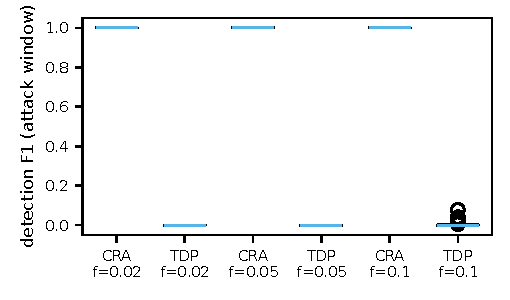
\includegraphics[width=\columnwidth]{e1_collapse.pdf}
\caption{E1: legacy Beta trust, node-detection F1 over the attack window (30 seeds).}\label{fig:e1}\end{figure}

\subsection{E2: SleeperGuard against sleepers}
SleeperGuard is better than legacy Beta in detection F1 in \EtwoSigBetter{} of \EtwoCells{} grid cells
(coalition $\times$ switch time $\times$ intensity; Holm-corrected paired Wilcoxon), worse in \EtwoSigWorse{}.
Median detection delay is \EtwoSgDelayMed{} steps versus \EtwoLgDelayMed{} for legacy Beta. The gain is
not uniform: against a \emph{stealthy} sleeper that inverts only 25\% of its votes, median F1 is about one half
(lowest cell median \EtwoSgFOneMin{}; Table~\ref{tab:e2}, Fig.~\ref{fig:e2}), because a node that lies rarely keeps
its Beta trust above 0.5 and is flagged only while quarantined. Invalid commits stayed rare for both
(max per-run rate \EtwoSgInvalid{} vs.\ \EtwoLgInvalid{}): with $\theta=0.667$ and at most 6 of 16 adversaries, the
main damage of this attack is to liveness (valid transactions rejected), which SleeperGuard reduces.
\begin{table}[t]
\centering\scriptsize
\caption{E2: legacy Beta vs SleeperGuard under the sleeper attack (t\_switch=300, honest fault 0.05), median [95\% CI] over 30 seeds. All grid cells and paired tests: results/raw/stats/e2\_sleeperguard.csv.}\label{tab:e2}
\resizebox{\columnwidth}{!}{%
\begin{tabular}{lllllll}
\toprule
coalition & intensity & F1 legacy & F1 SleeperGuard & delay SG (steps) & valid-reject legacy & valid-reject SG \\
\midrule
0.125 & 0.250000 & 0.000 [0.000, 0.000] & 0.484 [0.447, 0.527] & 5.000 [3.750, 6.000] & 0.001 [0.001, 0.001] & 0.001 [0.001, 0.001] \\
0.125 & 1.000000 & 0.000 [0.000, 0.000] & 0.975 [0.973, 0.985] & 0.000 [0.000, 0.750] & 0.004 [0.004, 0.005] & 0.000 [0.000, 0.001] \\
0.188 & 0.250000 & 0.000 [0.000, 0.000] & 0.492 [0.455, 0.517] & 7.000 [5.000, 9.500] & 0.006 [0.005, 0.007] & 0.003 [0.002, 0.003] \\
0.188 & 1.000000 & 0.000 [0.000, 0.000] & 0.989 [0.983, 0.991] & 0.000 [0.000, 1.000] & 0.017 [0.016, 0.018] & 0.001 [0.000, 0.001] \\
0.25 & 0.250000 & 0.000 [0.000, 0.000] & 0.467 [0.453, 0.500] & 6.500 [5.500, 8.500] & 0.030 [0.029, 0.031] & 0.008 [0.007, 0.009] \\
0.25 & 1.000000 & 0.000 [0.000, 0.000] & 0.992 [0.986, 0.994] & 0.000 [0.000, 1.000] & 0.064 [0.061, 0.065] & 0.003 [0.002, 0.003] \\
0.312 & 0.250000 & 0.000 [0.000, 0.000] & 0.477 [0.453, 0.501] & 7.000 [3.500, 8.000] & 0.108 [0.106, 0.110] & 0.023 [0.021, 0.028] \\
0.312 & 1.000000 & 0.000 [0.000, 0.000] & 0.993 [0.990, 0.994] & 0.000 [0.000, 1.000] & 0.215 [0.208, 0.217] & 0.003 [0.003, 0.004] \\
0.375 & 0.250000 & 0.000 [0.000, 0.000] & 0.484 [0.476, 0.515] & 5.750 [5.000, 8.000] & 0.250 [0.245, 0.253] & 0.055 [0.052, 0.061] \\
0.375 & 1.000000 & 0.000 [0.000, 0.000] & 0.994 [0.991, 0.995] & 0.000 [0.000, 1.000] & 0.536 [0.527, 0.542] & 0.006 [0.005, 0.007] \\
\bottomrule
\end{tabular}
}
\end{table}

\begin{figure}[t]\centering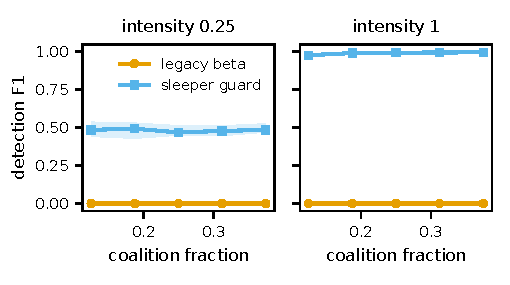
\includegraphics[width=\columnwidth]{e2_sleeperguard.pdf}
\caption{E2: detection F1 vs.\ coalition fraction (median, IQR band), middle switch time.}\label{fig:e2}\end{figure}

\subsection{E3: which component matters}
Against the stealthy sleeper, removing CUSUM drops median F1 from \EthreeFullFOne{} to \EthreeNoCusumFOne{} and raises
mean delay from \EthreeFullDelay{} to \EthreeNoCusumDelay{} steps; removing the two-timescale memory (\EthreeNoTwoFOne{})
or the share cap (\EthreeNoCapFOne{}) changes detection little; removing all three gives \EthreeNoneFOne{}
(Table~\ref{tab:e3}). CUSUM is the active ingredient; the cap matters for the safety bound, not for detection.
The adaptive attacker that replaces the earlier on-off attacker is evaluated in E11.
\begin{table}[t]
\centering\scriptsize
\caption{E3: SleeperGuard ablation, median [95\% CI] over 30 seeds. FQ = honest false quarantines per 1000 node-steps. Paired tests vs full: results/raw/stats/e3\_ablation.csv.}\label{tab:e3}
\resizebox{\columnwidth}{!}{%
\begin{tabular}{lllllll}
\toprule
attack & variant & F1 & delay & honest FQ/1000 & valid-reject & invalid-commit \\
\midrule
CRA (1) & full & 0.995 [0.995, 0.997] & 0.000 [0.000, 0.000] & 0.303 [0.152, 0.303] & 0.001 [0.001, 0.002] & 0.000 [0.000, 0.000] \\
CRA (1) & no-cusum & 1.000 [1.000, 1.000] & 0.000 [0.000, 0.000] & 0.000 [0.000, 0.000] & 0.002 [0.001, 0.002] & 0.000 [0.000, 0.000] \\
CRA (1) & no-two-timescale & 0.995 [0.995, 0.997] & 0.000 [0.000, 0.000] & 0.303 [0.152, 0.303] & 0.001 [0.001, 0.002] & 0.000 [0.000, 0.000] \\
CRA (1) & no-cap & 0.995 [0.995, 0.997] & 0.000 [0.000, 0.000] & 0.303 [0.152, 0.303] & 0.001 [0.001, 0.002] & 0.000 [0.000, 0.000] \\
CRA (1) & none & 1.000 [1.000, 1.000] & 0.000 [0.000, 0.000] & 0.000 [0.000, 0.000] & 0.002 [0.001, 0.002] & 0.000 [0.000, 0.000] \\
TDP (0.25) & full & 0.477 [0.453, 0.501] & 6.300 [4.300, 8.200] & 0.303 [0.227, 0.455] & 0.023 [0.021, 0.028] & 0.000 [0.000, 0.000] \\
TDP (0.25) & no-cusum & 0.047 [0.033, 0.061] & 66.700 [54.800, 90.100] & 0.000 [0.000, 0.000] & 0.058 [0.055, 0.063] & 0.000 [0.000, 0.000] \\
TDP (0.25) & no-two-timescale & 0.472 [0.448, 0.492] & 6.300 [4.300, 8.200] & 0.303 [0.227, 0.455] & 0.020 [0.018, 0.021] & 0.000 [0.000, 0.000] \\
TDP (0.25) & no-cap & 0.477 [0.453, 0.501] & 6.300 [4.300, 8.200] & 0.303 [0.227, 0.455] & 0.023 [0.021, 0.028] & 0.000 [0.000, 0.000] \\
TDP (0.25) & none & 0.000 [0.000, 0.000] & 300.000 [300.000, 300.000] & 0.000 [0.000, 0.000] & 0.056 [0.053, 0.060] & 0.000 [0.000, 0.000] \\
TDP (1) & full & 0.993 [0.990, 0.994] & 0.000 [0.000, 0.800] & 0.303 [0.227, 0.455] & 0.003 [0.003, 0.004] & 0.000 [0.000, 0.000] \\
TDP (1) & no-cusum & 0.998 [0.998, 0.998] & 1.000 [1.000, 1.400] & 0.000 [0.000, 0.000] & 0.004 [0.003, 0.004] & 0.000 [0.000, 0.000] \\
TDP (1) & no-two-timescale & 0.986 [0.983, 0.987] & 0.000 [0.000, 0.800] & 0.303 [0.227, 0.455] & 0.003 [0.003, 0.004] & 0.000 [0.000, 0.000] \\
TDP (1) & no-cap & 0.993 [0.990, 0.994] & 0.000 [0.000, 0.800] & 0.303 [0.227, 0.455] & 0.003 [0.003, 0.004] & 0.000 [0.000, 0.000] \\
TDP (1) & none & 0.930 [0.927, 0.934] & 39.400 [37.400, 41.000] & 0.000 [0.000, 0.000] & 0.034 [0.032, 0.036] & 0.000 [0.000, 0.000] \\
\bottomrule
\end{tabular}
}
\end{table}


\subsection{E4: cost and accuracy of the homomorphic tally}
Over \EfourDecisionsTotal{} random-instance decisions HETally disagreed with the plaintext rule \EfourFlipsTotal{}
times. In the guard-band stress test, decisions agreed for all $|m|\ge$\,\EfourBandMinSafe{} and flips occurred only at
$|m|\le$\,\EfourBandMaxFlip{} (including exact ties). A tally of $k=16$, $T=32$ takes a median \EfourMsZero{}~ms with raw
margins and \EfourMsThree{}~ms with three sign iterations (Table~\ref{tab:e4}, Fig.~\ref{fig:e4}); end-to-end, a step
costs \EfourConsWallZero{}~ms with HE ($s=0$) versus \EfourConsWallPlain{}~ms in plaintext, with
\EfourConsFlipsZero{} decision flips. \textbf{Negative result:} the sign iterations do not hide the margins.
Inverting $p^{(s)}$ recovers every margin to within \EfourLeakErrMax{}, and at most \EfourSatMaxPct{}\% of outputs are
saturated, so the decryptor learns margins in every configuration. The extra iterations add cost without a
measurable privacy gain at these margin magnitudes.
\begin{table}[t]
\centering\scriptsize
\caption{E4: HETally accuracy and cost (CKKS, TenSEAL). Flips = decisions differing from the plaintext rule; m = normalised margin. Latency: median [95\% CI] per tally on the machine in meta.json.}\label{tab:e4}
\resizebox{\columnwidth}{!}{%
\begin{tabular}{lllllllll}
\toprule
sign iters & N & modulus bits (max) & decisions & flips |m|>1e-3 & flips |m|<=1e-3 & max |m| of a flip & ms/tally k=16,T=32 & ct KB \\
\midrule
0 & 8192 & 160 (218) & 3360 & 0 & 0 & 0.00e+00 & 37.554 [35.881, 39.122] & 128 \\
1 & 16384 & 240 (438) & 3360 & 0 & 0 & 0.00e+00 & 221.039 [155.983, 241.716] & 256 \\
2 & 16384 & 320 (438) & 3360 & 0 & 0 & 0.00e+00 & 304.000 [276.540, 433.832] & 256 \\
3 & 16384 & 400 (438) & 3360 & 0 & 0 & 0.00e+00 & 451.207 [415.353, 503.456] & 256 \\
\bottomrule
\end{tabular}
}
\end{table}

\begin{table}[t]
\centering\scriptsize
\caption{E4b: end-to-end runs (TDP, SleeperGuard, 200 steps) with the plaintext vs HE tally on identical seeds.}\label{tab:e4b}
\resizebox{\columnwidth}{!}{%
\begin{tabular}{llllllll}
\toprule
sign iters & backend & seeds & F1 & invalid-commit & valid-reject & HE flips & wall ms/step \\
\midrule
0 & he & 5 & 0.588 [0.538, 0.603] & 0.000 [0.000, 0.000] & 0.020 [0.016, 0.030] & 0 & 32.172 [31.361, 33.035] \\
0 & plain & 5 & 0.588 [0.538, 0.603] & 0.000 [0.000, 0.000] & 0.020 [0.016, 0.030] & 0 & 0.493 [0.295, 0.604] \\
3 & he & 3 & 0.597 [0.538, 0.603] & 0.000 [0.000, 0.000] & 0.021 [0.016, 0.030] & 0 & 471.287 [465.047, 622.256] \\
3 & plain & 3 & 0.597 [0.538, 0.603] & 0.000 [0.000, 0.000] & 0.021 [0.016, 0.030] & 0 & 0.299 [0.225, 0.328] \\
\bottomrule
\end{tabular}
}
\end{table}

\begin{figure}[t]\centering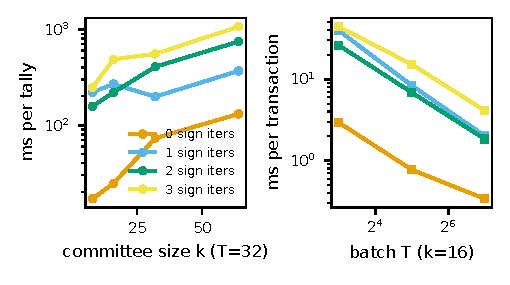
\includegraphics[width=\columnwidth]{e4_he_latency.pdf}
\caption{E4: HETally latency vs.\ committee size and per-transaction cost vs.\ batch size.}\label{fig:e4}\end{figure}

\subsection{E5: scale}
Simulation cost stays small (\EfiveBigWall{}~ms per step and \EfiveBigMem{}~MB peak heap at \EfiveMaxNodes{} nodes, $k=64$),
but \emph{detection does not scale with a fixed committee}: evidence about a node arrives only when it sits on the
committee, so at \EfiveMaxNodes{} nodes \EfiveBigCensoredPct{}\% of sleepers were never flagged within 300 steps (vs.\
\EfiveSmallCensoredPct{}\% at 16 nodes), and the worst cell has median F1 \EfiveMinFOne{} (Table~\ref{tab:e5}).
\begin{table}[t]
\centering\footnotesize\setlength{\tabcolsep}{4pt}
\caption{E5: scale, median over 30 seeds. p95 = simulated step latency (cost model, D7); wall = measured wall-clock per step; heap = peak Python heap of one run. Simulated throughput and p50/p99 latency: results/raw/e5\_scale/runs.csv.}\label{tab:e5}
\begin{tabular}{rrlrrr}
\toprule
$N$ & $k$ & F1 [95\% CI] & p95 ms & wall ms & heap MB \\
\midrule
16 & 8 & 0.83 [0.81, 0.85] & 20.2 & 2.00 & 2 \\
16 & 16 & 0.48 [0.45, 0.50] & 29.8 & 2.49 & 2 \\
64 & 8 & 0.65 [0.60, 0.69] & 20.2 & 2.30 & 3 \\
64 & 16 & 0.82 [0.80, 0.84] & 29.8 & 3.01 & 3 \\
64 & 32 & 0.83 [0.82, 0.85] & 68.2 & 3.47 & 3 \\
64 & 64 & 0.48 [0.47, 0.50] & 221.8 & 5.07 & 4 \\
256 & 8 & 0.24 [0.20, 0.26] & 20.2 & 2.25 & 9 \\
256 & 16 & 0.40 [0.39, 0.43] & 29.8 & 2.53 & 10 \\
256 & 32 & 0.66 [0.65, 0.68] & 68.2 & 3.65 & 10 \\
256 & 64 & 0.81 [0.80, 0.83] & 221.8 & 5.82 & 10 \\
1024 & 8 & 0.06 [0.05, 0.07] & 20.2 & 4.74 & 34 \\
1024 & 16 & 0.12 [0.11, 0.13] & 29.8 & 5.58 & 35 \\
1024 & 32 & 0.22 [0.21, 0.23] & 68.2 & 6.45 & 35 \\
1024 & 64 & 0.42 [0.38, 0.44] & 221.8 & 8.36 & 35 \\
\bottomrule
\end{tabular}
\end{table}


\subsection{E6: audit budget}
Detection degrades gracefully with the audit rate: at audit rate \EsixLowAudit{} SleeperGuard reaches median F1
\EsixSgFOneLowAudit{} against the stealthy sleeper, with mean delay \EsixSgDelayLowAudit{} steps versus \EsixSgDelayFullAudit{}
with every transaction audited (Fig.~\ref{fig:e6}).
\begin{figure}[t]\centering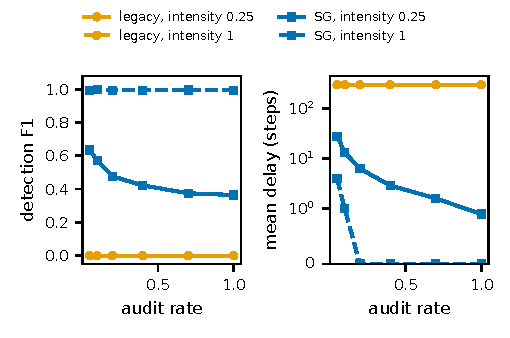
\includegraphics[width=\columnwidth]{e6_audit.pdf}
\caption{E6: detection F1 and delay vs.\ audit rate (median over 30 seeds).}\label{fig:e6}\end{figure}

\subsection{E7: the cost of false quarantines}
With CUSUM calibrated to the true honest fault rate, honest false quarantines per 1000 node-steps are \EsevenFqTwo{},
\EsevenFqFive{}, \EsevenFqTen{} and \EsevenFqTwenty{} at fault rates 0.02, 0.05, 0.10 and 0.20; calibrations for 0.15 and
0.20 lie outside the calibration grid's fault rates and use the nearest (0.10). Misspecified for 0.05 when the true
rate is 0.20, the rate rises to \EsevenFqMisTwenty{} and the valid-reject rate to \EsevenVrMisTwenty{} (Table~\ref{tab:e7}).
Fig.~\ref{fig:e7} shows the delay/false-quarantine trade-off as the alarm threshold varies.
\begin{table}[t]
\centering\scriptsize
\caption{E7: false-positive cost of SleeperGuard vs honest fault rate. 'matched': CUSUM calibrated for the true fault rate; 'fixed\_0.05': calibrated for 0.05 regardless (misspecified). Median [95\% CI], 30 seeds.}\label{tab:e7}
\resizebox{\columnwidth}{!}{%
\begin{tabular}{lllllll}
\toprule
honest fault & calibration & FQ/1000 (no attack) & valid-reject (no attack) & abort rate & F1 (TDP 0.25) & delay (TDP) \\
\midrule
0.000000 & fixed\_0.05 & 0.000 [0.000, 0.000] & 0.000 [0.000, 0.000] & 0.000 [0.000, 0.000] & 0.489 [0.421, 0.509] & 7.000 [4.500, 8.500] \\
0.000000 & matched & 0.000 [0.000, 0.000] & 0.000 [0.000, 0.000] & 0.000 [0.000, 0.000] & 0.678 [0.656, 0.689] & 3.500 [2.000, 4.500] \\
0.020000 & fixed\_0.05 & 0.000 [0.000, 0.000] & 0.000 [0.000, 0.000] & 0.000 [0.000, 0.000] & 0.487 [0.446, 0.512] & 6.400 [4.300, 8.200] \\
0.020000 & matched & 0.365 [0.312, 0.417] & 0.000 [0.000, 0.000] & 0.000 [0.000, 0.000] & 0.673 [0.644, 0.690] & 3.300 [2.000, 5.500] \\
0.050000 & fixed\_0.05 & 0.312 [0.208, 0.312] & 0.000 [0.000, 0.000] & 0.000 [0.000, 0.000] & 0.477 [0.453, 0.501] & 6.300 [4.300, 8.200] \\
0.050000 & matched & 0.312 [0.208, 0.312] & 0.000 [0.000, 0.000] & 0.000 [0.000, 0.000] & 0.477 [0.453, 0.501] & 6.300 [4.300, 8.200] \\
0.100000 & fixed\_0.05 & 2.188 [1.979, 2.448] & 0.006 [0.006, 0.006] & 0.000 [0.000, 0.000] & 0.487 [0.470, 0.503] & 5.900 [3.800, 7.400] \\
0.100000 & matched & 0.625 [0.469, 0.625] & 0.004 [0.004, 0.005] & 0.000 [0.000, 0.000] & 0.386 [0.358, 0.411] & 8.300 [7.000, 13.400] \\
0.150000 & fixed\_0.05 & 5.000 [4.896, 5.104] & 0.040 [0.039, 0.041] & 0.000 [0.000, 0.000] & 0.486 [0.468, 0.496] & 5.300 [3.800, 7.900] \\
0.150000 & matched & 1.927 [1.667, 2.083] & 0.033 [0.032, 0.034] & 0.000 [0.000, 0.000] & 0.414 [0.398, 0.431] & 10.200 [7.300, 14.000] \\
0.200000 & fixed\_0.05 & 8.073 [7.812, 8.385] & 0.122 [0.121, 0.123] & 0.000 [0.000, 0.000] & 0.502 [0.467, 0.520] & 5.900 [4.200, 7.200] \\
0.200000 & matched & 3.594 [3.333, 3.906] & 0.109 [0.108, 0.111] & 0.000 [0.000, 0.000] & 0.461 [0.442, 0.472] & 9.200 [7.000, 12.200] \\
\bottomrule
\end{tabular}
}
\end{table}

\begin{figure}[t]\centering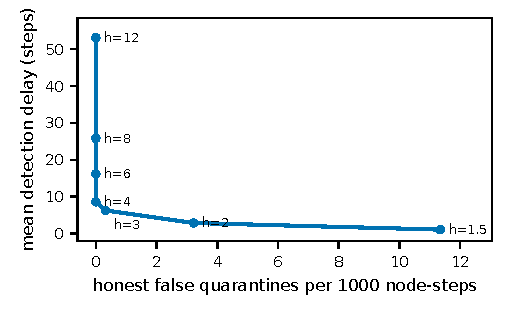
\includegraphics[width=\columnwidth]{e7_tradeoff.pdf}
\caption{E7: detection delay vs.\ honest false quarantines for CUSUM thresholds $h$.}\label{fig:e7}\end{figure}

\subsection{E8 (negative result): hiding the weights does not hinder bribery}
We tested the hypothesis that hiding trust weights hinders an adaptive briber; it is not supported. A briber that sees only the public ledger ranks delegates by how often their votes match
the committed outcome; this reaches a bribed weight share close to that of a briber who sees the weights (largest gap in median share \EeightMaxShareGap{}), and in
\EeightSig{} of \EeightTests{} (backend $\times$ budget) comparisons did the damage (valid-reject rate) differ significantly
after Holm correction. The ledger-based ranking beat random targeting in weight share in \EeightVotesBeatRandom{} of
\EeightVotesRandomTests{} cells (Table~\ref{tab:e8}). Public votes leak influence; encrypting weights alone does not hide it.
\begin{table}[t]
\centering\scriptsize
\caption{E8 (H3): bribery with public weights ('weights') vs hidden weights inferred from the public ledger ('votes') vs random targets. Share = bribed nodes' weight share at bribe time; valid-reject in the 40 steps after bribery. Median [95\% CI], 30 seeds; tests in results/raw/stats/e8\_privacy.csv.}\label{tab:e8}
\resizebox{\columnwidth}{!}{%
\begin{tabular}{llllllll}
\toprule
trust & B & share: weights & share: votes & share: random & valid-reject: weights & valid-reject: votes & valid-reject: random \\
\midrule
legacy beta & 2 & 0.251 [0.251, 0.252] & 0.251 [0.250, 0.251] & 0.125 [0.125, 0.125] & 0.259 [0.249, 0.265] & 0.261 [0.256, 0.268] & 0.047 [0.038, 0.053] \\
legacy beta & 3 & 0.377 [0.376, 0.377] & 0.376 [0.375, 0.376] & 0.250 [0.249, 0.251] & 1.000 [1.000, 1.000] & 1.000 [1.000, 1.000] & 0.260 [0.240, 0.283] \\
legacy beta & 4 & 0.502 [0.502, 0.502] & 0.501 [0.500, 0.501] & 0.374 [0.250, 0.375] & 1.000 [1.000, 1.000] & 1.000 [1.000, 1.000] & 0.939 [0.267, 1.000] \\
sleeper guard & 2 & 0.260 [0.258, 0.263] & 0.250 [0.246, 0.254] & 0.129 [0.122, 0.194] & 0.012 [0.011, 0.015] & 0.013 [0.012, 0.015] & 0.009 [0.006, 0.013] \\
sleeper guard & 3 & 0.390 [0.386, 0.392] & 0.373 [0.321, 0.377] & 0.248 [0.190, 0.292] & 0.035 [0.027, 0.038] & 0.029 [0.026, 0.034] & 0.017 [0.013, 0.028] \\
sleeper guard & 4 & 0.518 [0.513, 0.520] & 0.429 [0.375, 0.502] & 0.371 [0.268, 0.375] & 0.041 [0.036, 0.050] & 0.036 [0.031, 0.043] & 0.034 [0.020, 0.038] \\
\bottomrule
\end{tabular}
}
\end{table}


\subsection{E9: learning vs.\ rules}
All controllers were frozen and evaluated on unseen seeds. The factored independent learners obtained the highest
median reward (\EnineBestLearnerReward{} vs.\ \EnineRuleReward{} for the tuned rule and \EnineFixedReward{} for the fixed
SleeperGuard configuration; Table~\ref{tab:e9}, Fig.~\ref{fig:e9}), and \EnineLearnersBeatRule{} of the three learners beat the rule
significantly. D3P was not significantly better than the rule (reward \EnineDthreeReward{}). \textbf{Caveat:} the reward
(D8) values audited agreement, latency and audit cost, not detection. The best-reward learner shrinks committees and
audits and pays for it with a median detection delay of \EnineBestLearnerDelay{} steps versus \EnineFixedDelay{} for the fixed
configuration, and static DPoS, which detects nothing, scores \EnineDposReward{}. Higher reward here does not mean better
security; a reward that prices detection delay is future work.
\begin{table}[t]
\centering\scriptsize
\caption{E9: frozen controllers on eval seeds 100-129 pooled over six attack settings (180 runs each). Reward is the observable objective (D8); F1 excludes the no-attack setting. Median [95\% CI].}\label{tab:e9}
\resizebox{\columnwidth}{!}{%
\begin{tabular}{llllll}
\toprule
controller & reward & F1 & invalid-commit & valid-reject & throughput (sim.) \\
\midrule
pbft & 0.827 [0.790, 0.857] & 0.000 [0.000, 0.000] & 0.000 [0.000, 0.000] & 0.050 [0.005, 0.108] & 437 \\
static dpos & 0.913 [0.891, 0.922] & 0.000 [0.000, 0.000] & 0.000 [0.000, 0.000] & 0.034 [0.024, 0.068] & 741 \\
majority & 0.859 [0.859, 0.859] & 0.000 [0.000, 0.000] & 0.005 [0.004, 0.005] & 0.000 [0.000, 0.000] & 462 \\
random delegates & 0.864 [0.830, 0.894] & 0.000 [0.000, 0.000] & 0.001 [0.001, 0.002] & 0.099 [0.056, 0.154] & 685 \\
legacy beta & 0.843 [0.823, 0.857] & 0.000 [0.000, 0.000] & 0.000 [0.000, 0.000] & 0.025 [0.005, 0.051] & 450 \\
sleeper guard & 0.857 [0.856, 0.858] & 0.596 [0.548, 0.646] & 0.000 [0.000, 0.000] & 0.005 [0.003, 0.011] & 459 \\
sleeper guard fixed & 0.857 [0.856, 0.858] & 0.596 [0.548, 0.646] & 0.000 [0.000, 0.000] & 0.005 [0.003, 0.011] & 459 \\
rule & 0.856 [0.846, 0.861] & 0.632 [0.559, 0.682] & 0.000 [0.000, 0.000] & 0.015 [0.012, 0.024] & 424 \\
tabular q & 0.904 [0.903, 0.905] & 0.546 [0.422, 0.621] & 0.000 [0.000, 0.000] & 0.016 [0.013, 0.017] & 636 \\
d3p & 0.872 [0.867, 0.876] & 0.656 [0.612, 0.727] & 0.000 [0.000, 0.000] & 0.047 [0.044, 0.049] & 587 \\
marl factored & 0.920 [0.919, 0.922] & 0.693 [0.593, 0.777] & 0.000 [0.000, 0.000] & 0.019 [0.018, 0.021] & 764 \\
\bottomrule
\end{tabular}
}
\end{table}

\begin{figure}[t]\centering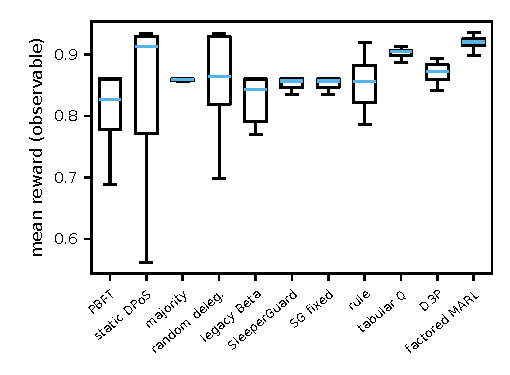
\includegraphics[width=\columnwidth]{e9_controllers.pdf}
\caption{E9: observable reward of frozen controllers on evaluation seeds.}\label{fig:e9}\end{figure}

\subsection{E10: the safety bound under adversarial search}
Across \EtenCells{} (k, c, $\theta$, b) cells the search found \EtenViolations{} violations of
Proposition~\ref{prop:safety} with the exact cap, and every one of the \EtenUnsafeCells{} cells the bound marks unsafe was
broken, so the bound is tight on this grid (Table~\ref{tab:e10}). With the original iterative cap, the tally's cap check
aborted \EtenIterAbortFrac{} of search candidates (exact cap: \EtenExactAbortFrac{}, all from infeasible weight
vectors); safety held only because of the abort.

\textbf{Direct test against the adaptive coalition (E10b).} In the full environment with the exact cap, the
damage-maximising coalition of E11 approved invalid transactions in coordination at lie rates 0.1, 0.3 and 1.0.
For coalitions the bound marks safe ($b\le5$ of 16), no run committed an invalid transaction: \EtenEnvBreachSafeZero{} of
\EtenEnvRunsSafeZero{} runs without honest faults and \EtenEnvBreachSafeFive{} of \EtenEnvRunsSafeFive{} with honest fault
rate 0.05. Above the bound ($b\ge6$), \EtenEnvBreachUnsafe{} of \EtenEnvRunsUnsafe{} runs committed at least one invalid
transaction (max rate \EtenEnvMaxInvalidUnsafe{}), all of them with honest faults present: the faulty honest approvals
are what carry an above-bound coalition over $\theta$, as the faults clause of the proposition predicts. The proposition
therefore needed no change; its honest-fault term is not vacuous (Table~\ref{tab:e10b}).
\begin{table}[t]
\centering\scriptsize
\caption{E10: adversarial search against the capped-influence bound (paper/proof.md). A violation = a commit forced with b below the bound.}\label{tab:e10}
\resizebox{\columnwidth}{!}{%
\begin{tabular}{llllll}
\toprule
k & c & theta & bound: safe for b <= & smallest b that forced a commit & violations \\
\midrule
8 & 1.500000 & 0.500000 & 2 & 3 & 0 \\
8 & 1.500000 & 0.667000 & 3 & 4 & 0 \\
8 & 1.500000 & 0.800000 & 4 & 5 & 0 \\
8 & 2.000000 & 0.500000 & 1 & 2 & 0 \\
8 & 2.000000 & 0.667000 & 2 & 3 & 0 \\
8 & 2.000000 & 0.800000 & 3 & 4 & 0 \\
8 & 3.000000 & 0.500000 & 1 & 2 & 0 \\
8 & 3.000000 & 0.667000 & 1 & 2 & 0 \\
8 & 3.000000 & 0.800000 & 2 & 3 & 0 \\
16 & 1.500000 & 0.500000 & 5 & 6 & 0 \\
16 & 1.500000 & 0.667000 & 7 & 8 & 0 \\
16 & 1.500000 & 0.800000 & 8 & 9 & 0 \\
16 & 2.000000 & 0.500000 & 3 & 4 & 0 \\
16 & 2.000000 & 0.667000 & 5 & 6 & 0 \\
16 & 2.000000 & 0.800000 & 6 & 7 & 0 \\
16 & 3.000000 & 0.500000 & 2 & 3 & 0 \\
16 & 3.000000 & 0.667000 & 3 & 4 & 0 \\
16 & 3.000000 & 0.800000 & 4 & 5 & 0 \\
32 & 1.500000 & 0.500000 & 10 & 11 & 0 \\
32 & 1.500000 & 0.667000 & 14 & 15 & 0 \\
32 & 1.500000 & 0.800000 & 17 & 18 & 0 \\
32 & 2.000000 & 0.500000 & 7 & 8 & 0 \\
32 & 2.000000 & 0.667000 & 10 & 11 & 0 \\
32 & 2.000000 & 0.800000 & 12 & 13 & 0 \\
32 & 3.000000 & 0.500000 & 5 & 6 & 0 \\
32 & 3.000000 & 0.667000 & 7 & 8 & 0 \\
32 & 3.000000 & 0.800000 & 8 & 9 & 0 \\
\bottomrule
\end{tabular}
}
\end{table}

\begin{table}[t]
\centering\scriptsize
\caption{E10b: full environment, exact cap ($k=16$, $c=2$, $	heta=0.667$; bound safe for $b\le5$), damage-maximising coalition approving invalid transactions at lie rates 0.1/0.3/1.0, 30 seeds each.}\label{tab:e10b}
\resizebox{\columnwidth}{!}{%
\begin{tabular}{llllll}
\toprule
b & honest fault & bound says safe & runs with an invalid commit & max invalid-commit rate & median F1 \\
\midrule
1 & 0.000000 & True & 0/9 & 0.0000 & 0.28 \\
1 & 0.050000 & True & 0/9 & 0.0000 & 0.21 \\
2 & 0.000000 & True & 0/9 & 0.0000 & 0.17 \\
2 & 0.050000 & True & 0/9 & 0.0000 & 0.11 \\
3 & 0.000000 & True & 0/9 & 0.0000 & 0.19 \\
3 & 0.050000 & True & 0/9 & 0.0000 & 0.06 \\
4 & 0.000000 & True & 0/9 & 0.0000 & 0.17 \\
4 & 0.050000 & True & 0/9 & 0.0000 & 0.17 \\
5 & 0.000000 & True & 0/9 & 0.0000 & 0.33 \\
5 & 0.050000 & True & 0/9 & 0.0000 & 0.08 \\
6 & 0.000000 & False & 0/9 & 0.0000 & 0.16 \\
6 & 0.050000 & False & 0/9 & 0.0000 & 0.10 \\
7 & 0.000000 & False & 0/9 & 0.0000 & 0.20 \\
7 & 0.050000 & False & 0/9 & 0.0000 & 0.10 \\
8 & 0.000000 & False & 0/9 & 0.0000 & 0.17 \\
8 & 0.050000 & False & 4/9 & 0.0014 & 0.04 \\
\bottomrule
\end{tabular}
}
\end{table}


\subsection{E11: a damage-maximising adaptive coalition}
For each defence we searched lie rate (0.05--1.0), coalition size (2--8 of 16) and target (approve invalid only, or
invert) on seeds 30--39 and kept the configuration with the highest invalid-commit rate. Against every defence the search
chose the largest coalition (\EelevenBSgFull{} of 16, i.e.\ above the bound) approving invalid transactions, at lie rate
\EelevenRateSgFull{} against full SleeperGuard (Table~\ref{tab:e11}). On evaluation seeds the median invalid-commit rate
was \EelevenInvalidSgFull{} with full SleeperGuard versus \EelevenInvalidLegacyBeta{} with legacy Beta and
\EelevenInvalidSgNone{} with all SleeperGuard components removed. \textbf{SleeperGuard does not detect this attacker
well}: median F1 \EelevenFOneSgFull{} (legacy Beta \EelevenFOneLegacyBeta{}; without CUSUM \EelevenFOneSgNoCusum{}). What
limits the damage is coalition size, not detection: for coalitions below the bound, full SleeperGuard had
\EelevenSgBelowBoundBreach{} invalid commits in \EelevenSgBelowBoundRuns{} runs.
\begin{table}[t]
\centering\scriptsize
\caption{E11: each defence against the damage-maximising coalition chosen by search on seeds 30-39 (lie rate, coalition size b of 16, target), evaluated on seeds 100-129. Median [95\% CI].}\label{tab:e11}
\resizebox{\columnwidth}{!}{%
\begin{tabular}{llllllll}
\toprule
defence & attacker lie rate & b & target & invalid-commit & valid-reject & F1 & runs w/ invalid commit \\
\midrule
legacy beta & 0.500000 & 8 & invalid & 0.002 [0.002, 0.003] & 0.000 [0.000, 0.000] & 0.000 [0.000, 0.000] & 30/30 \\
sg full & 0.500000 & 8 & invalid & 0.001 [0.000, 0.001] & 0.001 [0.000, 0.001] & 0.240 [0.224, 0.253] & 26/30 \\
sg no cusum & 0.500000 & 8 & invalid & 0.001 [0.001, 0.001] & 0.000 [0.000, 0.000] & 0.003 [0.002, 0.005] & 30/30 \\
sg no two timescale & 0.300000 & 8 & invalid & 0.001 [0.001, 0.001] & 0.000 [0.000, 0.000] & 0.129 [0.114, 0.142] & 28/30 \\
sg no cap & 0.500000 & 8 & invalid & 0.001 [0.000, 0.001] & 0.000 [0.000, 0.001] & 0.240 [0.224, 0.253] & 26/30 \\
sg none & 0.300000 & 8 & invalid & 0.001 [0.001, 0.002] & 0.000 [0.000, 0.000] & 0.000 [0.000, 0.000] & 29/30 \\
\bottomrule
\end{tabular}
}
\end{table}


\subsection{E12: detection versus lie rate}
With CUSUM calibrated on seeds 20--29 only, SleeperGuard's median F1 rises from \EtwelveFOneLow{} at lie rate
\EtwelveLowRate{} to \EtwelveFOneHigh{} at lie rate 1.0, first reaching 0.5 at lie rate \EtwelveHalfRate{}; legacy Beta
detects nothing below lie rate 0.75. The honest false-quarantine rate on the same runs stays at a median of at most
\EtwelveFqMax{} per 1000 node-steps across all lie rates (Fig.~\ref{fig:e12}). An attacker that lies on fewer than
\EtwelveHalfRate{} of its votes is therefore detected less than half the time.
\begin{figure}[t]\centering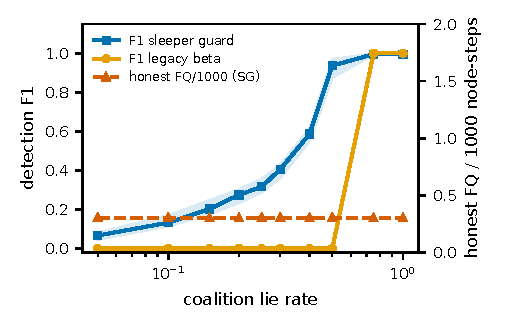
\includegraphics[width=\columnwidth]{e12_lierate.pdf}
\caption{E12: detection F1 (left axis, median and IQR) and honest false quarantines (right axis) vs.\ coalition lie rate.}\label{fig:e12}\end{figure}


\section{Limitations}
\begin{itemize}
\item \textbf{Simulation only.} Votes, faults and attacks are synthetic; the cost model is illustrative.
\item \textbf{Single key holder.} HETally runs all parties in one process with one secret key. A deployment
needs threshold or multiparty CKKS.
\item \textbf{Leakage.} The decryptor recovers the margins in every configuration we ran (E4) and, from a few
decrypted batches and the public votes, the trust weights themselves (E15), so the HE tally hides weights from the
aggregator but not from the decryptor.
\item \textbf{Unpredictable audits.} An adversary that predicts which transactions will be audited is not modelled.
Imperfect audits (wrong verdicts, delayed verdicts) are tested only at the rates in E16, with SleeperGuard not
re-calibrated for audit noise.
\item \textbf{Sub-threshold attackers.} A coalition that knows the CUSUM parameters can lie at a rate the
detector tolerates (E11, E12); the share cap, not detection, is then the only protection.
\item \textbf{Calibration.} SleeperGuard's CUSUM parameters depend on the nominal honest fault rate; E7 reports
the cost of misspecification.
\item \textbf{Simple detectors win on stealthy sleepers.} A fixed-reference CUSUM or EWMA detects the stealthy sleeper
better than SleeperGuard when the fault rate is known (E14); SleeperGuard's detection contribution is robustness to
misspecification, not detection power.
\item \textbf{Prior work read from abstracts.} The relation to~\cite{muniswamy2025trust} must be checked
against its full text.
\end{itemize}

\section{Conclusion}
Oracle access in a trust simulator changes conclusions. Measured without it, a Beta-reputation trust model
fails against sleepers; change detection recovers detection of attackers that lie often, at a stated
false-quarantine cost, but not of attackers that lie below the alarm rate; an exactly enforced weight cap gives a
safety bound that held against every adversary we tried within its assumptions; and a homomorphic tally
reproduces the plaintext decisions at a measured cost while revealing margins to its decryptor.

\bibliographystyle{IEEEtran}
\bibliography{refs}
\end{document}
